% Baylor University Thesis LaTeX template
% - Template created by Jonathan Drake (2013)
% - Template updated by Kenneth Call, Kenichi Hatakeyama (2019)
% - Template updated by Chris Madrid, Caleb Smith (2020)

% Thesis class, based on report
\documentclass
[
	%short,	% omit front matter
	%draft, % draft heading, don't load graphics, etc.
]
{thesis}

% Optional additional packages
\usepackage{appendix}
\usepackage{etoolbox}
\usepackage{graphicx}
\usepackage{epstopdf}
\usepackage{amsmath}
\usepackage{chicago}
\usepackage{lipsum} % Because this comes with a demo
%\usepackage[hang, flushmargin, symbol]{footmisc}
\usepackage[hyperfootnotes=false, hidelinks=true]{hyperref}  % for workin links and bookmarks (alexsalo)
\usepackage[capitalise,nameinlink]{cleveref}  % used to format references to ranges of references.
\usepackage{bookmark}  % faster bookmarks manegment (alexsalo)
\usepackage{ifthen}
\usepackage[binary-units]{siunitx} %Easier use of scientific notation (Check also CMS defined units)
%\usepackage{topcapt} %This lets us put the table caption at the top using \topcaption
\usepackage{amssymb}
\usepackage{acronym} %This is used to create the List of acronyms
\usepackage[nobreak]{cite}
\usepackage{xspace}
\usepackage{xcolor}
\usepackage{slashed}
\usepackage{pdfpages}
\usepackage[textsize=footnotesize,textwidth=2.7cm]{todonotes}
\usepackage{footnotebackref}
\usepackage{adjustbox}
\usepackage{rotating}
\usepackage{tabu}

%%KC: Graduate school asks that references to chapters use words for the numbers. the fmtcount package translates number to words. This is really rather hacky. If the formated label is an integer according to xstring, then we set the hackyCounter to have that label's value, then print it using \Numberstring
\usepackage{fmtcount, xstring}

\newcount\hackyCounter
\newcounter{hackyCounter}

\creflabelformat{chapter}{#2\IfInteger{#1}{\setcounter{hackyCounter}{#1}\Numberstring{hackyCounter}}{#1}#3}

% using cleveref for appendices
% https://tex.stackexchange.com/questions/119513/cleveref-and-appendix-packages-appendix-referenced-as-section
\AtBeginEnvironment{appendices}{\crefalias{chapter}{appendix}}

%%special commands
%\setlength{\marginparwidth}{4cm}
\newcommand{\tinytodo}[2][]
{\todo[caption={#2}, #1]{\renewcommand{\baselinestretch}{0.8}\selectfont#2\par}}
\newcommand{\fxnote}[1]{\tinytodo{#1}}
\newcommand{\fixme}[1]{{\color{red}{FIXME: #1}}}
%\renewcommand{\footnote}[2][3]{\footnotemark[#1]\footnotetext[#1]{#2}}
\renewcommand{\chapterautorefname}{\mbox{Chapter}}
\renewcommand{\sectionautorefname}{\mbox{Section}}
\renewcommand{\subsectionautorefname}{\mbox{Section}}

%%Thesis parameters
\title{Electromagnetic and Hadronic Cluster Calibration for the CMS Particle Flow Algorithm Using Machine Learning Methods}    
%\title{Electromagnetic and Hadronic Cluster Calibration For CMS Experiment Particle Flow Reconstruction Using machine Learning Methods}
\author{Noorah Asaad Ghazwani}
\holding{B.S.}
\seeking{M.S.}
\degree{Master of Science}
\project{A Thesis}
\date{July 2024}

%% Administration
\graduateDean{J.~Larry Lyon, Ph.D.}
\department{Department of Physics}
\departmentChair{Lorin Swint Matthews, Ph.D.}
\departmentChairTitle{Chairperson}

%% Supervisor (advisor / mentor)
\supervisor{Kenichi Hatakeyam, Ph.D.}
\supervisorRole{Advisor}

%% Readers (committee members)
\committee{Dissertation Committee}
\readerOne{Kenichi Hatakeyama Ph.D., Chairperson}
\readerTwo{Jay R. Dittmann, Ph.D.}
\readerThree{Andrew Brinkerhoff, Ph.D.}
\readerFour{not decided yet.}


%% CMS specific commands
%% \def\Fileversion$#1: #2 ${\gdef\fileversion{#2}}
%% \def\Filedate$#1: #2-#3-#4 #5 ${\gdef\filedate{#2/#3/#4}}
%% \Fileversion$Revision: 452536 $
%% \Filedate$Date: 2018-03-25 12:00:22 -0500 (Sun, 25 Mar 2018) $
%% %%%%%%%%%%%%%%%%%%%%%%%%%%%%%%%%%%%%%%%%%%%%%%%%%%%%%%%%%%%%%%%%%%%%
%% %
%% %  CMS Common definitions style file
%% %
%% %  N.B. use of \newcommand rather than \newcommand means
%% %       that a definition is ignored if already specified
%% %
%% %                                              L. Taylor 18 Feb 2005
%% %%%%%%%%%%%%%%%%%%%%%%%%%%%%%%%%%%%%%%%%%%%%%%%%%%%%%%%%%%%%%%%%%%%%
%% \NeedsTeXFormat{LaTeX2e}
%% \ProvidesPackage{ptdr-definitions}[\filedate\space CMS Additional Macro Definitions (\fileversion)]
\RequirePackage{xspace}
\RequirePackage{amsmath}

% Some shorthand
% turn off italics
\newcommand {\etal}{\mbox{et al.}\xspace} %et al. - no preceding comma
\newcommand {\ie}{\mbox{i.e.}\xspace}     %i.e.
\newcommand {\eg}{\mbox{e.g.}\xspace}     %e.g.
\newcommand {\etc}{\mbox{etc.}\xspace}     %etc.
\newcommand {\aka}{\mbox{aka.}\xspace}     %aka.
\newcommand {\vs}{\mbox{\sl vs.}\xspace}      %vs.
\newcommand {\mdash}{\ensuremath{\mathrm{-}}} % for use within formulas
\providecommand {\NA}{\ensuremath{\text{---}}}    % for Not applicable (or available). Needs to be renewcommanded for APS to \cdots

% some terms whose definition we may change
\newcommand {\Lone}{Level-1\xspace} % Level-1 or L1 ?
\newcommand {\Ltwo}{Level-2\xspace}
\newcommand {\Lthree}{Level-3\xspace}

% Some software programs (alphabetized)
\newcommand{\ACERMC} {\textsc{AcerMC}\xspace}
\newcommand{\ALPGEN} {{\textsc{alpgen}}\xspace}
\newcommand{\BLACKHAT} {{\textsc{BlackHat}}\xspace}
\newcommand{\CALCHEP} {{\textsc{CalcHEP}}\xspace}
\newcommand{\CHARYBDIS} {{\textsc{charybdis}}\xspace}
\newcommand{\CMKIN} {\textsc{cmkin}\xspace}
\newcommand{\CMSIM} {{\textsc{cmsim}}\xspace}
\newcommand{\CMSSW} {{\textsc{cmssw}}\xspace}
\newcommand{\COBRA} {{\textsc{cobra}}\xspace}
\newcommand{\COCOA} {{\textsc{cocoa}}\xspace}
\newcommand{\COMPHEP} {\textsc{CompHEP}\xspace}
\newcommand{\EVTGEN} {{\textsc{evtgen}}\xspace}
\newcommand{\FAMOS} {{\textsc{famos}}\xspace}
\newcommand{\FASTJET} {{\textsc{FastJet}}\xspace}
\newcommand{\FEWZ} {{\textsc{fewz}}\xspace}
\newcommand{\GARCON} {\textsc{garcon}\xspace}
\newcommand{\GARFIELD} {{\textsc{garfield}}\xspace}
\newcommand{\GEANE} {{\textsc{geane}}\xspace}
\newcommand{\GEANTfour} {{\textsc{Geant4}}\xspace}
\newcommand{\GEANTthree} {{\textsc{geant3}}\xspace}
\newcommand{\GEANT} {{\textsc{geant}}\xspace}
\newcommand{\HDECAY} {\textsc{hdecay}\xspace}
\newcommand{\HERWIG} {{\textsc{herwig}}\xspace}
\newcommand{\HERWIGpp} {{\textsc{herwig++}}\xspace}
\newcommand{\POWHEG} {{\textsc{powheg}}\xspace}
\newcommand{\HIGLU} {{\textsc{higlu}}\xspace}
\newcommand{\HIJING} {{\textsc{hijing}}\xspace}
\newcommand{\HYDJET} {{\textsc{hydjet}}\xspace}
\newcommand{\IGUANA} {\textsc{iguana}\xspace}
\newcommand{\ISAJET} {{\textsc{isajet}}\xspace}
\newcommand{\ISAPYTHIA} {{\textsc{isapythia}}\xspace}
\newcommand{\ISASUGRA} {{\textsc{isasugra}}\xspace}
\newcommand{\ISASUSY} {{\textsc{isasusy}}\xspace}
\newcommand{\ISAWIG} {{\textsc{isawig}}\xspace}
\newcommand{\MADGRAPH} {\textsc{MadGraph}\xspace}
\newcommand{\MCATNLO} {\textsc{mc@nlo}\xspace}
\newcommand{\MCFM} {\textsc{mcfm}\xspace}
\newcommand{\MILLEPEDE} {{\textsc{millepede}}\xspace}
\newcommand{\ORCA} {{\textsc{orca}}\xspace}
\newcommand{\OSCAR} {{\textsc{oscar}}\xspace}
\newcommand{\PHOTOS} {\textsc{photos}\xspace}
\newcommand{\PROSPINO} {\textsc{prospino}\xspace}
\newcommand{\PYTHIA} {{\textsc{pythia}}\xspace}
\newcommand{\SHERPA} {{\textsc{sherpa}}\xspace}
\newcommand{\TAUOLA} {\textsc{tauola}\xspace}
\newcommand{\TOPREX} {\textsc{TopReX}\xspace}
\newcommand{\XDAQ} {{\textsc{xdaq}}\xspace}
\newcommand{\MGvATNLO}{\MADGRAPH{}5\_a\MCATNLO}


%  Experiments
\newcommand {\DZERO}{D0\xspace}     %etc.


% Measurements and units...

\newcommand{\de}{\ensuremath{^\circ}}
\newcommand{\ten}[1]{\ensuremath{\times \text{10}^\text{#1}}}
\newcommand{\unit}[1]{\ensuremath{\text{\ #1}}\xspace}
\newcommand{\mum}{\ensuremath{\ \mu\text{m}}\xspace}
\newcommand{\micron}{\ensuremath{\ \mu\text{m}}\xspace}
\newcommand{\cm}{\ensuremath{\ \text{cm}}\xspace}
\newcommand{\mm}{\ensuremath{\ \text{mm}}\xspace}
\newcommand{\second}{\ensuremath{\ \text{s}}\xspace}
\newcommand{\mus}{\ensuremath{\ \mu\text{s}}\xspace}
\newcommand{\keV}{\ensuremath{\ \text{ke\hspace{-.08em}V}}\xspace}
\newcommand{\MeV}{\ensuremath{\ \text{Me\hspace{-.08em}V}}\xspace}
\newcommand{\MeVns}{\ensuremath{\text{Me\hspace{-.08em}V}}\xspace} % no leading thinspace
\newcommand{\GeV}{\ensuremath{\ \text{Ge\hspace{-.08em}V}}\xspace}
\newcommand{\GeVns}{\ensuremath{\text{Ge\hspace{-.08em}V}}\xspace} % no leading thinspace
\newcommand{\gev}{\GeV}
\newcommand{\TeV}{\ensuremath{\ \text{Te\hspace{-.08em}V}}\xspace}
\newcommand{\TeVns}{\ensuremath{\text{Te\hspace{-.08em}V}}\xspace} % no leading thinspace
\newcommand{\PeV}{\ensuremath{\ \text{Pe\hspace{-.08em}V}}\xspace}
\newcommand{\keVc}{\ensuremath{{\ \text{ke\hspace{-.08em}V\hspace{-0.16em}/\hspace{-0.08em}}c}}\xspace}
\newcommand{\MeVc}{\ensuremath{{\ \text{Me\hspace{-.08em}V\hspace{-0.16em}/\hspace{-0.08em}}c}}\xspace}
\newcommand{\GeVc}{\ensuremath{{\ \text{Ge\hspace{-.08em}V\hspace{-0.16em}/\hspace{-0.08em}}c}}\xspace}
\newcommand{\GeVcns}{\ensuremath{{\text{Ge\hspace{-.08em}V\hspace{-0.16em}/\hspace{-0.08em}}c}}\xspace} % no leading thinspace
\newcommand{\TeVc}{\ensuremath{{\ \text{Te\hspace{-.08em}V\hspace{-0.16em}/\hspace{-0.08em}}c}}\xspace}
\newcommand{\keVcc}{\ensuremath{{\ \text{ke\hspace{-.08em}V\hspace{-0.16em}/\hspace{-0.08em}}c^\text{2}}}\xspace}
\newcommand{\MeVcc}{\ensuremath{{\ \text{Me\hspace{-.08em}V\hspace{-0.16em}/\hspace{-0.08em}}c^\text{2}}}\xspace}
\newcommand{\GeVcc}{\ensuremath{{\ \text{Ge\hspace{-.08em}V\hspace{-0.16em}/\hspace{-0.08em}}c^\text{2}}}\xspace}
\newcommand{\GeVccns}{\ensuremath{{\text{Ge\hspace{-.08em}V\hspace{-0.16em}/\hspace{-0.08em}}c^\text{2}}}\xspace} % no leading thinspace
\newcommand{\TeVcc}{\ensuremath{{\ \text{Te\hspace{-.08em}V\hspace{-0.16em}/\hspace{-0.08em}}c^\text{2}}}\xspace}

\newcommand{\mb}{\ensuremath{\ \text{mb}}\xspace}
\newcommand{\mub}{\ensuremath{\ \mu\text{b}}\xspace}
\newcommand{\nbarn}{\ensuremath{\ \text{nb}}\xspace}
\newcommand{\pb}{\ensuremath{\ \text{pb}}\xspace}
\newcommand{\fb}{\ensuremath{\ \text{fb}}\xspace}
\newcommand{\mbinv}{\ensuremath{\ \text{mb}^{-1}}\xspace}
\newcommand{\mubinv}{\ensuremath{\ \mu\text{b}^{-1}}\xspace}
\newcommand{\nbinv}{\ensuremath{\ \text{nb}^{-1}}\xspace}
\newcommand{\pbinv}{\ensuremath{\ \text{pb}^{-1}}\xspace}
\newcommand{\fbinv}{\ensuremath{\ \text{fb}^{-1}}\xspace}
\newcommand{\percms}{\ensuremath{\ \text{cm}^\text{$-$2}\ \text{s}^\text{$-$1}}\xspace}
\newcommand{\lumi}{\ensuremath{\mathcal{L}}\xspace}
\newcommand{\Lumi}{\lumi}
\newcommand{\rate}{\ensuremath{\mathcal{R}}\xspace}
\newcommand{\Rate}{\rate}

% Need a convention here:
\newcommand{\LvLow}  {\ensuremath{\mathcal{L}=\text{10}^\text{32}\,\text{cm}^\text{$-$2}\,\text{s}^\text{$-$1}}\xspace}
\newcommand{\LLow}   {\ensuremath{\mathcal{L}=\text{10}^\text{33}\,\text{cm}^\text{$-$2}\,\text{s}^\text{$-$1}}\xspace}
\newcommand{\lowlumi}{\ensuremath{\mathcal{L}=\text{2}\times \text{10}^\text{33}\,\text{cm}^\text{$-$2}\,\text{s}^\text{$-$1}}\xspace}
\newcommand{\LMed}   {\ensuremath{\mathcal{L}=\text{2}\times \text{10}^\text{33}\,\text{cm}^\text{$-$2}\,\text{s}^\text{$-$1}}\xspace}
\newcommand{\LHigh}  {\ensuremath{\mathcal{L}=\text{10}^\text{34}\,\text{cm}^\text{$-$2}\,\text{s}^\text{$-$1}}\xspace}
\newcommand{\hilumi} {\ensuremath{\mathcal{L}=\text{10}^\text{34}\,\text{cm}^\text{$-$2}\,\text{s}^\text{$-$1}}\xspace}

% Physics symbols ...
\newcommand{\PT}{\ensuremath{p_{\mathrm{T}}}\xspace}
\newcommand{\pt}{\PT}
\newcommand{\pT}{\PT}
\newcommand{\ET}{\ensuremath{E_{\mathrm{T}}}\xspace}
\newcommand{\HT}{\ensuremath{H_{\mathrm{T}}}\xspace}
\newcommand{\et}{\ensuremath{E_{\mathrm{T}}}\xspace}
\newcommand{\Em}{\ensuremath{E\hspace{-0.6em}/}\xspace}
\newcommand{\Pm}{\ensuremath{p\hspace{-0.5em}/}\xspace}
\newcommand{\PTm}{\ensuremath{{p}_\mathrm{T}\hspace{-1.02em}/\kern 0.5em}\xspace}
\newcommand{\PTslash}{\PTm}
\newcommand{\ETm}{\ensuremath{E_{\mathrm{T}}^{\text{miss}}}\xspace}
\newcommand{\MET}{\ensuremath{p^{\rm miss}_{\rm T}}\xspace}
\newcommand{\METv}{\ensuremath{\vec{p}^{\rm miss}_{\rm T}}\xspace}
\newcommand{\ETmiss}{\ETm}
\newcommand{\ptmiss}{\ensuremath{\pt^\text{miss}}\xspace}
\newcommand{\ETslash}{\ensuremath{E_{\mathrm{T}}\hspace{-1.1em}/\kern0.45em}\xspace}
\newcommand{\VEtmiss}{\ensuremath{{\vec E}_{\mathrm{T}}^{\text{miss}}}\xspace}
\newcommand{\ptvec}{\ensuremath{{\vec p}_{\mathrm{T}}}\xspace}
\newcommand{\ptvecmiss}{\ensuremath{{\vec p}_{\mathrm{T}}^{\kern1pt\text{miss}}}\xspace}
\newcommand{\tauh}{\ensuremath{\PGt_\mathrm{h}}\xspace}
\newcommand{\sqrtsNN}{\ensuremath{\sqrt{\smash[b]{s_{_{\mathrm{NN}}}}}}\xspace}
\newcommand{\mht}{\ensuremath{H_{\mathrm{T}}^{\text{miss}}}\xspace}
\newcommand{\htvecmiss}{\ensuremath{\vec{H}_{\text{T}}^{\text{miss}}}\xspace}
\newcommand{\dphi}{\ensuremath{\Delta\phi}\xspace}
\newcommand{\MTTwo}{\ensuremath{m_{\text{T2}}}\xspace}
\newcommand{\mt}{\ensuremath{m_{\mathrm{T}}}\xspace}
\newcommand{\mT}{\mt}
\newcommand{\Mt}{\mt}
\newcommand{\MT}{\mt}
\newcommand{\mtb}{\ensuremath{\mt^\mathrm{\PQb}}\xspace}
\newcommand{\MTb}{\mtb}
\newcommand{\mTb}{\mtb}
\newcommand{\ptb}{\ensuremath{\pt^{\mathrm{\PQb}}}\xspace}
\newcommand{\ptbonetwo}{\ensuremath{\pt^{\mathrm{\PQb}_{12}}}}
\newcommand{\ptISR}{\ensuremath{\pt^{\text{ISR}}}\xspace}

\newcommand{\metsig}{\ensuremath{\ptmiss/\sqrt{H_\mathrm{T}}}\xspace}
\newcommand{\sipthreed}{{\tt SIP3D}\xspace}

% aliases to existing commands
\newcommand{\ptisr}{\ptISR}
\newcommand{\Ht}{\HT}
\newcommand{\met}{\MET}
\newcommand{\metv}{\METv}
\newcommand{\vMet}{\METv}
\newcommand{\vmet}{\METv}

% roman face derivative
\newcommand{\dd}[2]{\ensuremath{\frac{\cmsSymbolFace{d} #1}{\cmsSymbolFace{d} #2}}}
\newcommand{\ddinline}[2]{\ensuremath{\cmsSymbolFace{d} #1/\cmsSymbolFace{d} #2}}
\newcommand{\rd}{\ensuremath{\cmsSymbolFace{d}}}
\newcommand{\re}{\ensuremath{\cmsSymbolFace{e}}}
% absolute value
\newcommand{\abs}[1]{\ensuremath{\lvert #1 \rvert}}
% misc
\newcommand{\CL}{\ensuremath{\text{CL}}\xspace}
\newcommand{\CLs}{\ensuremath{\text{CL}_\text{s}}\xspace}
\newcommand{\CLsb}{\ensuremath{\text{CL}_\text{s+b}}\xspace}


%%%KH \ifthenelse{\boolean{cms@italic}}{\newcommand{\cmsSymbolFace}[1]{#1}}{\newcommand{\cmsSymbolFace}[1]{\mathrm{#1}}}
\newcommand{\cmsSymbolFace}[1]{\mathrm{#1}}

% Particle names which track the italic/non-italic face convention
\newcommand{\zp}{\ensuremath{{\cmsSymbolFace{Z}^\prime}}\xspace} % plain Z'
\newcommand{\JPsi}{\ensuremath{{\cmsSymbolFace{J}\hspace{-.08em}/\hspace{-.14em}\psi}}\xspace} % J/Psi (no mass)
\newcommand{\Z}{\ensuremath{\cmsSymbolFace{Z}}\xspace} % plain Z (no superscript 0)
\newcommand{\ttbar}{\ensuremath{{\cmsSymbolFace{t}\overline{\cmsSymbolFace{t}}}}\xspace} % t-tbar

% Extensions for missing names in PENNAMES % note no xspace, to match syntax in PENNAMES
\newcommand{\cPgn}{\ensuremath{\nu}} % generic neutrino
\providecommand{\Pgn}{\ensuremath{\nu}} % generic neutrino
\newcommand{\cPagn}{\ensuremath{\overline{\nu}}} % generic neutrino
\providecommand{\Pagn}{\ensuremath{\overline{\nu}}} % generic neutrino
\newcommand{\cPgg}{\ensuremath{\gamma}} % gamma
\newcommand{\cPJgy}{\ensuremath{\cmsSymbolFace{J}\hspace{-.08em}/\hspace{-.14em}\psi}} % J/Psi (no mass)
\newcommand{\cPW}{\ensuremath{\cmsSymbolFace{W}}} % W, no xspace
\newcommand{\cPZ}{\ensuremath{\cmsSymbolFace{Z}}} % plain Z (no superscript 0), no xspace
\newcommand{\cPZpr}{\ensuremath{\cmsSymbolFace{Z}'}} % plain Z'
\newcommand{\cPqt}{\ensuremath{\cmsSymbolFace{t}}} % t for t quark
\newcommand{\cPqb}{\ensuremath{\cmsSymbolFace{b}}} % b for b quark
\newcommand{\cPqc}{\ensuremath{\cmsSymbolFace{c}}} % c for c quark
\newcommand{\cPqs}{\ensuremath{\cmsSymbolFace{s}}} % s for s quark
\newcommand{\cPqu}{\ensuremath{\cmsSymbolFace{u}}} % u for u quark
\newcommand{\cPqd}{\ensuremath{\cmsSymbolFace{d}}} % d for d quark
\newcommand{\cPq}{\ensuremath{\cmsSymbolFace{q}}} % generic quark
\newcommand{\cPg}{\ensuremath{\cmsSymbolFace{g}}} % generic gluon
\newcommand{\cPG}{\ensuremath{\cmsSymbolFace{G}}} % Graviton
\newcommand{\cPaqt}{\ensuremath{\overline{\cmsSymbolFace{t}}}} % t for t anti-quark
\newcommand{\cPaqb}{\ensuremath{\overline{\cmsSymbolFace{b}}}} % b for b anti-quark
\newcommand{\cPaqc}{\ensuremath{\overline{\cmsSymbolFace{c}}}} % c for c anti-quark
\newcommand{\cPaqs}{\ensuremath{\overline{\cmsSymbolFace{s}}}} % s for s anti-quark
\newcommand{\cPaqu}{\ensuremath{\overline{\cmsSymbolFace{u}}}} % u for u anti-quark
\newcommand{\cPaqd}{\ensuremath{\overline{\cmsSymbolFace{d}}}} % d for d anti-quark
\newcommand{\cPaq}{\ensuremath{\overline{\cmsSymbolFace{q}}}} % generic anti-quark
\newcommand{\cPKstz}{\ensuremath{\cmsSymbolFace{K}^{\ast0}}\xspace} %note has xspace
% future symbols from heppennames2
\providecommand{\PGp}{\ensuremath{\pi}\xspace} % pi
\providecommand{\PGpp}{\ensuremath{\pi^+}\xspace} % pi
\providecommand{\PGpm}{\ensuremath{\pi^-}\xspace} % pi
\providecommand{\PGpz}{\ensuremath{\pi^0}\xspace} % pi
\providecommand{\PGr}{\ensuremath{\rho}\xspace} % pi
\providecommand{\PDast}{\ensuremath{\cmsSymbolFace{D}^\ast}\xspace} % D star
\providecommand{\PH}{\ensuremath{\cmsSymbolFace{H}}\xspace} % plain Higgs
\providecommand{\Ph}{\ensuremath{\cmsSymbolFace{h}}\xspace} % SUSY Higgs
\providecommand{\Pa}{\ensuremath{\cmsSymbolFace{a}}\xspace}
\providecommand{\PSA}{\ensuremath{\cmsSymbolFace{A}}\xspace} %pseudoscalar A Higgs
\providecommand{\PJGy}{\ensuremath{\cmsSymbolFace{J}\hspace{-.08em}/\hspace{-.14em}\psi}\xspace} % J/Psi (no mass)
\providecommand{\PBzs}{\ensuremath{\cmsSymbolFace{B}^0_\cmsSymbolFace{s}}\xspace} % B^0_s
\providecommand{\Pg}{\ensuremath{\cmsSymbolFace{g}}\xspace} % generic gluon
\providecommand{\PSg}{\ensuremath{\widetilde{\cmsSymbolFace{g}}}\xspace} % gluino
\providecommand{\PSQ}{\ensuremath{\widetilde{\cmsSymbolFace{q}}}\xspace} % squark
\providecommand{\PSGm}{\ensuremath{\widetilde{\mu}}\xspace} % smuon
\providecommand{\PSe}{\ensuremath{\widetilde{\cmsSymbolFace{e}}}\xspace} % selectron
\providecommand{\PASQ}{\ensuremath{\overline{\widetilde{\cmsSymbolFace{q}}}}\xspace} % anti quark
\providecommand{\PXXA}{\ensuremath{\cmsSymbolFace{A}}\xspace} % axion
\providecommand{\PXXG}{\ensuremath{\cmsSymbolFace{G}}\xspace} % graviton
\providecommand{\PXXSG}{\ensuremath{\widetilde{\PXXG}}\xspace} % gravitino
\providecommand{\PSGcp}{\ensuremath{\widetilde{\chi}^+}\xspace} % lightest positive chargino
\providecommand{\PSGcm}{\ensuremath{\widetilde{\chi}^-}\xspace} % lightest negative chargino
\providecommand{\PSGc}{\ensuremath{\widetilde{\chi}}\xspace} % neutralino
\providecommand{\PSGcz}{\ensuremath{\widetilde{\chi}^0}\xspace} % neutralino with superscript 0
\providecommand{\PSGczDo}{\ensuremath{\widetilde{\chi}^{0}_{1}}\xspace} % neutralino
\providecommand{\PSGcmDo}{\ensuremath{\widetilde{\chi}^{-}_{1}}\xspace} % neutralino
\providecommand{\PSGczDt}{\ensuremath{\widetilde{\chi}^{0}_{2}}\xspace} % neutralino
\providecommand{\PSGcpm}{\ensuremath{\widetilde{\chi}^\pm}\xspace} % neutralino
\providecommand{\PSGcpmDo}{\ensuremath{\widetilde{\chi}^\pm_{1}}\xspace} % neutralino
\providecommand{\PSGcpDo}{\ensuremath{\widetilde{\chi}^{+}_{1}}\xspace} % neutralino
\providecommand{\Pl}{\ensuremath{\cmsSymbolFace{l}}\xspace} % non-ell lepton
\providecommand{\PAl}{\ensuremath{\overline{\cmsSymbolFace{l}}}\xspace} % non-ell anti-lepton
\providecommand{\PGnl}{\ensuremath{\nu_\cmsSymbolFace{l}}\xspace} % lepton neutrino
\providecommand{\PAGnl}{\ensuremath{\overline{\nu}_\cmsSymbolFace{l}}\xspace} % anti-lepton neutrino
\providecommand{\PQtpr}{\ensuremath{\cmsSymbolFace{t}^{\prime}}\xspace} % t'
\providecommand{\PAQtpr}{\ensuremath{\bar{\cmsSymbolFace{t}}^\prime}\xspace} % t'-bar; needs to be converted to overline-requires rework a la heppennames
\providecommand{\PQbpr}{\ensuremath{\cmsSymbolFace{b}^{\prime}}\xspace} % b'
\providecommand{\PAQbpr}{\ensuremath{\bar{\cmsSymbolFace{b}}^\prime}\xspace} % b'-bar; needs same as anti-t'
\providecommand{\PGg}{\ensuremath{\gamma}\xspace} % gamma
\providecommand{\PKzS}{\ensuremath{\cmsSymbolFace{K}^0_\cmsSymbolFace{S}}\xspace} % K short
\providecommand{\PBs}{\ensuremath{\cmsSymbolFace{B}_\cmsSymbolFace{s}}\xspace} % B sub s
\providecommand{\PSQu}{\ensuremath{\widetilde{\cmsSymbolFace{u}}}\xspace}
\providecommand{\PSQd}{\ensuremath{\widetilde{\cmsSymbolFace{d}}}\xspace}
\providecommand{\PSQc}{\ensuremath{\widetilde{\cmsSymbolFace{c}}}\xspace}
\providecommand{\PSQs}{\ensuremath{\widetilde{\cmsSymbolFace{s}}}\xspace}
\providecommand{\PSQt}{\ensuremath{\widetilde{\cmsSymbolFace{t}}}\xspace} % stop
\providecommand{\PSQb}{\ensuremath{\widetilde{\cmsSymbolFace{b}}}\xspace}
\providecommand{\PASQt}{\ensuremath{\overline{\widetilde{\cmsSymbolFace{t}}}}\xspace} % anti stop
\providecommand{\PASQb}{\ensuremath{\overline{\widetilde{\cmsSymbolFace{b}}}}\xspace} % anti sbottom
\providecommand{\PSGt}{\ensuremath{\widetilde{\tau}}\xspace} % stau
\providecommand{\PZ}{\ensuremath{\cmsSymbolFace{Z}}\xspace} % may have some confusion with the \xspace...
\providecommand{\PZpr}{\ensuremath{\cmsSymbolFace{Z}'}\xspace} % plain Z' using prime
\newcommand{\PW}{\ensuremath{\cmsSymbolFace{W}}\xspace} % use prime like pennames2
\newcommand{\WW}{\ensuremath{\cmsSymbolFace{W}\cmsSymbolFace{W}}\xspace}
\newcommand{\ZZ}{\ensuremath{\cmsSymbolFace{Z}\cmsSymbolFace{Z}}\xspace}
%%KH \renewcommand{\PWpr}{\ensuremath{\cmsSymbolFace{W}'}\xspace} % use prime like pennames2
\newcommand{\PWpr}{\ensuremath{\cmsSymbolFace{W}'}\xspace} % use prime like pennames2
\providecommand{\PWmp}{\ensuremath{\cmsSymbolFace{W}^\mp}\xspace}
\providecommand{\PDstp}{\ensuremath{\cmsSymbolFace{D}^{\ast+}}\xspace}
\providecommand{\PDstm}{\ensuremath{\cmsSymbolFace{D}^{\ast-}}\xspace}
\providecommand{\PGn}{\ensuremath{\nu}\xspace} % generic neutrino
\providecommand{\PAGn}{\ensuremath{\overline{\nu}}\xspace} % generic neutrino
\providecommand{\PSQtDo}{\ensuremath{\widetilde{\cmsSymbolFace{t}}_1}\xspace}
\providecommand{\PSQtDt}{\ensuremath{\widetilde{\cmsSymbolFace{t}}_2}\xspace}
\providecommand{\PQt}{\ensuremath{\cmsSymbolFace{t}}\xspace} % t
\providecommand{\PAQt}{\ensuremath{\overline{\cmsSymbolFace{t}}}\xspace} %
\providecommand{\PQb}{\ensuremath{\cmsSymbolFace{b}}\xspace} % b
\providecommand{\PAQb}{\ensuremath{\overline{\cmsSymbolFace{b}}}\xspace} %
\providecommand{\PGm}{\ensuremath{\mu}\xspace} % muon
\providecommand{\PGmm}{\ensuremath{\mu^-}\xspace} % muon
\providecommand{\PGmp}{\ensuremath{\mu^+}\xspace} % muon
\providecommand{\PGmpm}{\ensuremath{\mu^\pm}\xspace} % muon
\providecommand{\PGt}{\ensuremath{\tau}\xspace} % tau
\providecommand{\PAGt}{\ensuremath{\overline{\tau}}\xspace} % anti-tau
\providecommand{\PGpz}{\ensuremath{\pi^0}\xspace}
\providecommand{\PQq}{\ensuremath{\cmsSymbolFace{q}}\xspace} % quark (generic)
\providecommand{\PQd}{\ensuremath{\cmsSymbolFace{d}}\xspace} % down quark
\providecommand{\PQu}{\ensuremath{\cmsSymbolFace{u}}\xspace} % up quark
\providecommand{\PQs}{\ensuremath{\cmsSymbolFace{s}}\xspace} % top quark
\providecommand{\PQc}{\ensuremath{\cmsSymbolFace{c}}\xspace} % top quark
\providecommand{\PAQq}{\ensuremath{\overline{\cmsSymbolFace{q}}}\xspace} % quark (generic)
\providecommand{\PAQd}{\ensuremath{\overline{\cmsSymbolFace{d}}}\xspace} % down quark
\providecommand{\PAQu}{\ensuremath{\overline{\cmsSymbolFace{u}}}\xspace} % up quark
\providecommand{\PAQs}{\ensuremath{\overline{\cmsSymbolFace{s}}}\xspace} % top quark
\providecommand{\PAQc}{\ensuremath{\overline{\cmsSymbolFace{c}}}\xspace} % top quark
\providecommand{\PGne}{\ensuremath{\nu_\cmsSymbolFace{e}}\xspace} % electron neutrino
\providecommand{\PAGne}{\ensuremath{\overline{\nu}_\cmsSymbolFace{e}}\xspace} % anti-electron neutrino
\providecommand{\PAGe}{\ensuremath{\overline{\cmsSymbolFace{e}}}\xspace} % anti-electron
\providecommand{\PGnGm}{\ensuremath{\nu_\PGm}\xspace} % muon neutrino
\providecommand{\PAGnGm}{\ensuremath{\overline{\nu}_\PGm}\xspace} % anti-muon neutrino
\providecommand{\PGnGt}{\ensuremath{\nu_\PGt}\xspace} % tau neutrino
\providecommand{\PAGnGt}{\ensuremath{\overline{\nu}_\PGt}\xspace} % anti-tau neutrino
\providecommand{\PAp}{\ensuremath{\overline{\cmsSymbolFace{p}}}\xspace} % anti-proton
\providecommand{\PAn}{\ensuremath{\overline{\cmsSymbolFace{n}}}\xspace} % anti-neutron
\providecommand{\PGc}{\ensuremath{\chi}\xspace} % chi (charm, but also SUSY)
\providecommand{\PDz}{\ensuremath{\cmsSymbolFace{D}^0}\xspace} % D0 meson
\providecommand{\PADz}{\ensuremath{\overline{\cmsSymbolFace{D}}^0}\xspace} % anti-D0 meson
\providecommand{\PAD}{\ensuremath{\overline{\cmsSymbolFace{D}}}\xspace} % anti-D meson
\providecommand{\PAK}{\ensuremath{\overline{\cmsSymbolFace{K}}}\xspace} % anti-K meson
\providecommand{\PAKz}{\ensuremath{\overline{\cmsSymbolFace{K}}^0}\xspace} % anti-K0 meson
\providecommand{\PABz}{\ensuremath{\overline{\cmsSymbolFace{B}}^0}\xspace} % anti-B0 meson

% our extensions for pennames2
\providecommand{\Pepm}{\ensuremath{\cmsSymbolFace{e}^\pm}\xspace}
\providecommand{\Pemp}{\ensuremath{\cmsSymbolFace{e}^\mp}\xspace}
\providecommand{\PGmpm}{\ensuremath{\mu^\pm}\xspace}
\providecommand{\PGmmp}{\ensuremath{\mu^\mp}\xspace} % not available in pennames2, AFAIK

% for APS style tables

% \ifthenelse{\boolean{cms@external}}{
% \newenvironment{scotch}[1]{\protect\centering\ruledtabular\tabular{#1}}{\endtabular\endruledtabular}
% }{
% \newenvironment{scotch}[1]{\protect\centering\tabular{#1}}{\endtabular}
% \newenvironment{turnpage}[1]{#1}{}
% }

% \ifthenelse{\boolean{cms@external}}{
% \newenvironment{scotch}[1]{\protect\centering\ruledtabular\tabular{#1}}{\endtabular\endruledtabular}
% }{
% \newenvironment{scotch}[1]{\protect\centering\tabular{#1}\hline\hline}{\hline\endtabular}
% }

\newenvironment{scotch}[1]{\protect\centering\tabular{#1}\hline}{\hline\endtabular}

% Other
\newcommand{\MD}{\ensuremath{{M_\mathrm{D}}}\xspace}% ED mass
\newcommand{\Mpl}{\ensuremath{{M_\mathrm{Pl}}}\xspace}% Planck mass
\newcommand{\Rinv} {\ensuremath{{R}^{-1}}\xspace}

% SM (still to be classified)

\newcommand{\AFB}{\ensuremath{A_\text{FB}}\xspace}
\newcommand{\wangle}{\ensuremath{\sin^{2}\theta_{\text{eff}}^\text{lept}(M^2_{\Z})}\xspace}
\newcommand{\stat}{\ensuremath{\,\text{(stat)}}\xspace}
\newcommand{\syst}{\ensuremath{\,\text{(syst)}}\xspace}
\newcommand{\thy}{\ensuremath{\,\text{(theo)}}\xspace}
\newcommand{\lum}{\ensuremath{\,\text{(lumi)}}\xspace}
\newcommand{\kt}{\ensuremath{k_{\mathrm{T}}}\xspace}

\newcommand{\BC}{\ensuremath{\cmsSymbolFace{B_{c}}}\xspace}
\newcommand{\bbarc}{\ensuremath{\PQb\PAQc}\xspace}
\newcommand{\bbbar}{\ensuremath{\PQb\PAQb}\xspace}
\newcommand{\ccbar}{\ensuremath{\PQc\PAQc}\xspace}
\newcommand{\qqbar}{\ensuremath{\PQq\PAQq}\xspace}
\newcommand{\bspsiphi}{\ensuremath{\cmsSymbolFace{B_s} \to \JPsi\, \phi}\xspace}
\newcommand{\EE}{\ensuremath{\Pep\Pem}\xspace}
\newcommand{\MM}{\ensuremath{\Pgmp\Pgmm}\xspace}
\newcommand{\TT}{\ensuremath{\Pgt^{+}\Pgt^{-}}\xspace}

%%%  E-gamma definitions
\newcommand{\HGG}{\ensuremath{\cmsSymbolFace{H}\to\gamma\gamma}}
\newcommand{\GAMJET}{\ensuremath{\gamma + \text{jet}}}
\newcommand{\PPTOJETS}{\ensuremath{\Pp\Pp\to\text{jets}}}
\newcommand{\PPTOGG}{\ensuremath{\Pp\Pp\to\gamma\gamma}}
\newcommand{\PPTOGAMJET}{\ensuremath{\Pp\Pp\to\gamma + \text{jet}}}
\newcommand{\MH}{\ensuremath{M_{\PH}}}
\newcommand{\RNINE}{\ensuremath{R_\mathrm{9}}}
\newcommand{\DR}{\ensuremath{\Delta R}}





%%%%%%
% From Albert
%

\newcommand{\ga}{\ensuremath{\gtrsim}}
\newcommand{\la}{\ensuremath{\lesssim}}
%
\newcommand{\swsq}{\ensuremath{\sin^2\theta_\cmsSymbolFace{W}}\xspace}
\newcommand{\cwsq}{\ensuremath{\cos^2\theta_\cmsSymbolFace{W}}\xspace}
\newcommand{\tanb}{\ensuremath{\tan\beta}\xspace}
\newcommand{\tanbsq}{\ensuremath{\tan^{2}\beta}\xspace}
\newcommand{\sidb}{\ensuremath{\sin 2\beta}\xspace}
\newcommand{\alpS}{\ensuremath{\alpha_S}\xspace}
\newcommand{\alpt}{\ensuremath{\tilde{\alpha}}\xspace}

\newcommand{\QL}{\ensuremath{\cmsSymbolFace{Q}_\cmsSymbolFace{L}}\xspace}
\newcommand{\sQ}{\ensuremath{\widetilde{\cmsSymbolFace{Q}}}\xspace}
\newcommand{\sQL}{\ensuremath{\widetilde{\cmsSymbolFace{Q}}_\cmsSymbolFace{L}}\xspace}
\newcommand{\ULC}{\ensuremath{\cmsSymbolFace{U}_\cmsSymbolFace{L}^\cmsSymbolFace{C}}\xspace}
\newcommand{\sUC}{\ensuremath{\widetilde{\cmsSymbolFace{U}}^\cmsSymbolFace{C}}\xspace}
\newcommand{\sULC}{\ensuremath{\widetilde{\cmsSymbolFace{U}}_\cmsSymbolFace{L}^\cmsSymbolFace{C}}\xspace}
\newcommand{\DLC}{\ensuremath{\cmsSymbolFace{D}_\cmsSymbolFace{L}^\cmsSymbolFace{C}}\xspace}
\newcommand{\sDC}{\ensuremath{\widetilde{\cmsSymbolFace{D}}^\cmsSymbolFace{C}}\xspace}
\newcommand{\sDLC}{\ensuremath{\widetilde{\cmsSymbolFace{D}}_\cmsSymbolFace{L}^\cmsSymbolFace{C}}\xspace}
\newcommand{\LL}{\ensuremath{\cmsSymbolFace{L}_\cmsSymbolFace{L}}\xspace}
\newcommand{\sL}{\ensuremath{\widetilde{\cmsSymbolFace{L}}}\xspace}
\newcommand{\sLL}{\ensuremath{\widetilde{\cmsSymbolFace{L}}_\cmsSymbolFace{L}}\xspace}
\newcommand{\ELC}{\ensuremath{\cmsSymbolFace{E}_\cmsSymbolFace{L}^\cmsSymbolFace{C}}\xspace}
\newcommand{\sEC}{\ensuremath{\widetilde{\cmsSymbolFace{E}}^\cmsSymbolFace{C}}\xspace}
\newcommand{\sELC}{\ensuremath{\widetilde{\cmsSymbolFace{E}}_\cmsSymbolFace{L}^\cmsSymbolFace{C}}\xspace}
\newcommand{\sEL}{\ensuremath{\widetilde{\cmsSymbolFace{E}}_\cmsSymbolFace{L}}\xspace}
\newcommand{\sER}{\ensuremath{\widetilde{\cmsSymbolFace{E}}_\cmsSymbolFace{R}}\xspace}
\newcommand{\sFer}{\ensuremath{\widetilde{\cmsSymbolFace{f}}}\xspace}
\newcommand{\sQua}{\ensuremath{\widetilde{\cmsSymbolFace{q}}}\xspace}
\newcommand{\sUp}{\ensuremath{\widetilde{\cmsSymbolFace{u}}}\xspace}
\newcommand{\suL}{\ensuremath{\widetilde{\cmsSymbolFace{u}}_\cmsSymbolFace{L}}\xspace}
\newcommand{\suR}{\ensuremath{\widetilde{\cmsSymbolFace{u}}_\cmsSymbolFace{R}}\xspace}
\newcommand{\sDw}{\ensuremath{\widetilde{\cmsSymbolFace{d}}}\xspace}
\newcommand{\sdL}{\ensuremath{\widetilde{\cmsSymbolFace{d}}_\cmsSymbolFace{L}}\xspace}
\newcommand{\sdR}{\ensuremath{\widetilde{\cmsSymbolFace{d}}_\cmsSymbolFace{R}}\xspace}
\newcommand{\sTop}{\ensuremath{\widetilde{\cmsSymbolFace{t}}}\xspace}
\newcommand{\stL}{\ensuremath{\widetilde{\cmsSymbolFace{t}}_\cmsSymbolFace{L}}\xspace}
\newcommand{\stR}{\ensuremath{\widetilde{\cmsSymbolFace{t}}_\cmsSymbolFace{R}}\xspace}
\newcommand{\stone}{\ensuremath{\widetilde{\cmsSymbolFace{t}}_1}\xspace}
\newcommand{\sttwo}{\ensuremath{\widetilde{\cmsSymbolFace{t}}_2}\xspace}
\newcommand{\sBot}{\ensuremath{\widetilde{\cmsSymbolFace{b}}}\xspace}
\newcommand{\sbL}{\ensuremath{\widetilde{\cmsSymbolFace{b}}_\cmsSymbolFace{L}}\xspace}
\newcommand{\sbR}{\ensuremath{\widetilde{\cmsSymbolFace{b}}_\cmsSymbolFace{R}}\xspace}
\newcommand{\sbone}{\ensuremath{\widetilde{\cmsSymbolFace{b}}_1}\xspace}
\newcommand{\sbtwo}{\ensuremath{\widetilde{\cmsSymbolFace{b}}_2}\xspace}
\newcommand{\sLep}{\ensuremath{\widetilde{\cmsSymbolFace{l}}}\xspace}
\newcommand{\sLepC}{\ensuremath{\widetilde{\cmsSymbolFace{l}}^\cmsSymbolFace{C}}\xspace}
\newcommand{\sEl}{\ensuremath{\widetilde{\cmsSymbolFace{e}}}\xspace}
\newcommand{\sElC}{\ensuremath{\widetilde{\cmsSymbolFace{e}}^\cmsSymbolFace{C}}\xspace}
\newcommand{\seL}{\ensuremath{\widetilde{\cmsSymbolFace{e}}_\cmsSymbolFace{L}}\xspace}
\newcommand{\seR}{\ensuremath{\widetilde{\cmsSymbolFace{e}}_\cmsSymbolFace{R}}\xspace}
\newcommand{\snL}{\ensuremath{\widetilde{\nu}_L}\xspace}
\newcommand{\sMu}{\ensuremath{\widetilde{\mu}}\xspace}
\newcommand{\sNu}{\ensuremath{\widetilde{\nu}}\xspace}
\newcommand{\sTau}{\ensuremath{\widetilde{\tau}}\xspace}
\newcommand{\Glu}{\ensuremath{\cmsSymbolFace{g}}\xspace}
\newcommand{\sGlu}{\ensuremath{\widetilde{\cmsSymbolFace{g}}}\xspace}
\newcommand{\Wpm}{\ensuremath{\cmsSymbolFace{W}^{\pm}}\xspace}
\newcommand{\sWpm}{\ensuremath{\widetilde{\cmsSymbolFace{W}}^{\pm}}\xspace}
\newcommand{\Wz}{\ensuremath{\cmsSymbolFace{W}^{0}}\xspace}
\newcommand{\sWz}{\ensuremath{\widetilde{\cmsSymbolFace{W}}^{0}}\xspace}
\newcommand{\sWino}{\ensuremath{\widetilde{\cmsSymbolFace{W}}}\xspace}
\newcommand{\Bz}{\ensuremath{\cmsSymbolFace{B}^{0}}\xspace}
\newcommand{\sBz}{\ensuremath{\widetilde{\cmsSymbolFace{B}}^{0}}\xspace}
\newcommand{\sBino}{\ensuremath{\widetilde{\cmsSymbolFace{B}}}\xspace}
\newcommand{\Zz}{\ensuremath{\cmsSymbolFace{Z}^{0}}\xspace}
\newcommand{\sZino}{\ensuremath{\widetilde{\cmsSymbolFace{Z}}^{0}}\xspace}
\newcommand{\sGam}{\ensuremath{\widetilde{\gamma}}\xspace}
\newcommand{\chiz}{\ensuremath{\widetilde{\chi}^{0}}\xspace}
\newcommand{\chip}{\ensuremath{\widetilde{\chi}^{+}}\xspace}
\newcommand{\chim}{\ensuremath{\widetilde{\chi}^{-}}\xspace}
\newcommand{\chipm}{\ensuremath{\widetilde{\chi}^{\pm}}\xspace}
\newcommand{\Hone}{\ensuremath{\cmsSymbolFace{H}_\cmsSymbolFace{d}}\xspace}
\newcommand{\sHone}{\ensuremath{\widetilde{\cmsSymbolFace{H}}_\cmsSymbolFace{d}}\xspace}
\newcommand{\Htwo}{\ensuremath{\cmsSymbolFace{H}_\cmsSymbolFace{u}}\xspace}
\newcommand{\sHtwo}{\ensuremath{\widetilde{\cmsSymbolFace{H}}_\cmsSymbolFace{u}}\xspace}
\newcommand{\sHig}{\ensuremath{\widetilde{\cmsSymbolFace{H}}}\xspace}
\newcommand{\sHa}{\ensuremath{\widetilde{\cmsSymbolFace{H}}_\cmsSymbolFace{a}}\xspace}
\newcommand{\sHb}{\ensuremath{\widetilde{\cmsSymbolFace{H}}_\cmsSymbolFace{b}}\xspace}
\newcommand{\sHpm}{\ensuremath{\widetilde{\cmsSymbolFace{H}}^{\pm}}\xspace}
\newcommand{\hz}{\ensuremath{\cmsSymbolFace{h}^{0}}\xspace}
\newcommand{\Hz}{\ensuremath{\cmsSymbolFace{H}^{0}}\xspace}
\newcommand{\Az}{\ensuremath{\cmsSymbolFace{A}^{0}}\xspace}
\newcommand{\Hpm}{\ensuremath{\cmsSymbolFace{H}^{\pm}}\xspace}
\newcommand{\sGra}{\ensuremath{\widetilde{\cmsSymbolFace{G}}}\xspace}
%
\newcommand{\mtil}{\ensuremath{\widetilde{m}}\xspace}
%
\newcommand{\rpv}{\ensuremath{\rlap{\kern.2em/}R}\xspace}
\newcommand{\LLE}{\ensuremath{LL\bar{E}}\xspace}
\newcommand{\LQD}{\ensuremath{LQ\bar{D}}\xspace}
\newcommand{\UDD}{\ensuremath{\overline{UDD}}\xspace}
\newcommand{\Lam}{\ensuremath{\lambda}\xspace}
\newcommand{\Lamp}{\ensuremath{\lambda'}\xspace}
\newcommand{\Lampp}{\ensuremath{\lambda''}\xspace}
%
\newcommand{\spinbd}[2]{\ensuremath{\bar{#1}_{\dot{#2}}}\xspace}


%%%%%%% More definitions
\newcommand\defRTDR{\ensuremath{ R2 = \sqrt{[\pi-\Delta\phi(J_{1},\mht) ]^2 +[\Delta\phi(J_{2},\mht) ]^2}    }}
\newcommand\wpj{\ensuremath{\W + {\rm jets}}\xspace}
\newcommand\zpj{\ensuremath{\Z + {\rm jets}}\xspace}
\renewcommand{\ttbar}{\ensuremath{{\rm t\bar{t}}}\xspace}
\renewcommand\qqbar{\ensuremath{{\rm q\bar{q}}}\xspace}
\newcommand\ttbarMuNu{\ensuremath{\ttbar ( \mu \nu ) {\rm +jets}}\xspace}
\newcommand\wtauhad{\ensuremath{\W \rightarrow \tau_{\rm h} \nu}\xspace}
\newcommand\ttbarTAUHNu{\ensuremath{\ttbar \rightarrow \tau_{\rm h} \nu + {\rm jets}}\xspace}
\newcommand\ttbarDITAUHNu{\ensuremath{\ttbar \rightarrow \tau_{\rm h} \nu + \tau_{\rm h} \nu + {\rm jets}}\xspace}
\newcommand\ttbarMUTAUHNu{\ensuremath{\ttbar ( \mu \nu + \tau_{\mu} \nu) {\rm +jets}}\xspace}
\newcommand\defMHT{\ensuremath{ {\rm MHT} = \mht = | - \sum_{i} \vec{p_{T} (jet_{i}) }|}}
\newcommand{\ztautau}{\ensuremath{\Z \rightarrow \tau \tau}\xspace}
\newcommand{\zmumu}{\ensuremath{\Z \rightarrow \mu^{+} \mu^{-}}\xspace}
\newcommand{\zee}{\ensuremath{\Z \rightarrow \e^{+} \e^{-}}\xspace}
\newcommand{\znunu}{\ensuremath{\Z \rightarrow \nu \bar{\nu}}\xspace}
\newcommand{\zll}{\ensuremath{\Z \rightarrow \ell^{+}\ell^{-}}\xspace}
\newcommand{\wlnu}{\ensuremath{\W \rightarrow \ell\nu}\xspace}
\newcommand{\wenu}{\ensuremath{\W \rightarrow \e\nu}\xspace}
\newcommand{\wmunu}{\ensuremath{\W \rightarrow \mu \nu}\xspace}
\newcommand{\zellell}{\ensuremath{\Z \rightarrow \ell^{+} \ell^{-}}\xspace}
\newcommand{\znunubr}{\ensuremath{\Z ( \nu \bar{\nu} )}\xspace}
\newcommand{\zellellbr}{\ensuremath{\Z ( \ell^{+} \ell^{-} )}\xspace}
\newcommand{\wmunubr}{\ensuremath{\W (\mu \nu )}\xspace}
\newcommand{\wenubr}{\ensuremath{\W (\e\nu )}\xspace}
\newcommand{\wlnubr}{\ensuremath{\W (\ell \nu )}\xspace}
\newcommand{\wellnubr}{\ensuremath{\W (\ell \nu )}\xspace}
\newcommand{\wtaunubr} {\ensuremath{\W (\tau \nu )}\xspace}
\newcommand{\ztautaubr}{\ensuremath{\Z (\tau \tau)}\xspace}
\newcommand{\zmumubr}  {\ensuremath{\Z (\mu \mu)}\xspace}
\newcommand{\zeebr}    {\ensuremath{\Z (\e \e)}\xspace}
\newcommand{\tfll}     {\ensuremath{TF_\mathrm{LL}}\xspace}
\newcommand{\ttW}{\ensuremath{\ttbar{}\PW}\xspace}
\newcommand{\ttZ}{\ensuremath{\ttbar{}\PZ}\xspace}

% object counting
\newcommand{\Nj}{\ensuremath{N_{\text{j}}}\xspace}
\newcommand{\Nb}{\ensuremath{N_{\text{b}}}\xspace}
\newcommand{\Nsv}{\ensuremath{N_{\text{SV}}}\xspace}
\newcommand{\Nw}{\ensuremath{N_{\text{W}}}\xspace}
\newcommand{\Nt}{\ensuremath{N_{\text{t}}}\xspace}
\newcommand{\Nres}{\ensuremath{N_{\text{res}}}\xspace}
\newcommand{\Ntw}{\ensuremath{N_{\text{tW}}}\xspace}
% aliases to existing commands
\newcommand{\nj}{\Nj}
\newcommand{\nb}{\Nb}
\newcommand{\nsv}{\Nsv}
\newcommand{\nw}{\Nw}
\newcommand{\nt}{\Nt}
\newcommand{\nrt}{\Nres}
\newcommand{\ntw}{\Ntw}

% For Z invisible background
\newcommand{\metlepton}{\ensuremath{\pt^{\mathrm{miss} (LL)}}\xspace}
\newcommand{\metphoton}{\ensuremath{\pt^{\mathrm{miss} (\gamma)}}\xspace}
\newcommand{\DRphopar}{\ensuremath{\Delta R_{\gamma p}}\xspace}
\newcommand{\RZ}{\ensuremath{R_{\PZ}}\xspace}
\newcommand{\RT}{\ensuremath{R_{\mathrm{T}}}\xspace}
\newcommand{\SGamma}{\ensuremath{S_{\gamma}}\xspace}
\newcommand{\NMC}{\ensuremath{N_{\mathrm{MC}}^{\znunu}}\xspace}
\newcommand{\NP}{\ensuremath{N_{\mathrm{pred}}^{\znunu}}\xspace}
\newcommand{\Rz}{\RZ}
\newcommand{\rz}{\RZ}
\newcommand{\Rt}{\RT}
\newcommand{\rt}{\RT}
\newcommand{\SG}{\SGamma}
\newcommand{\Sg}{\SGamma}
\newcommand{\sg}{\SGamma}
\newcommand{\Nmc}{\NMC}
\newcommand{\nmc}{\NMC}
\newcommand{\Np}{\NP}
\newcommand{\np}{\NP}

\newcommand{\cmsTable}[1]{\resizebox{\textwidth}{!}{#1}}
\newlength\cmsTabSkip\setlength{\cmsTabSkip}{1ex}

%\endinput

\newcommand{\nbjets}{\ensuremath{N_{\PQb}}\xspace}
\newcommand{\njets}{\ensuremath{N_{\text{j}}}\xspace}
\newcommand{\ntops}{\ensuremath{N_{\PQt}}\xspace}
\newcommand{\htmiss}{\ensuremath{H_{\text{T}}^{\text{miss}}}\xspace}
\newcommand{\mbl}{\ensuremath{M(l,b)}\xspace}
\newcommand{\znunujets}{\ensuremath{\cPZ(\PGn\PAGn)}\text{+jets}\xspace}
\newcommand{\Znunujets}{\znunujets}
\newcommand{\zjets}{{{\cPZ}\text{+jets}}\xspace}
\newcommand{\wjets}{{{\PW}\text{+jets}}\xspace}
\newcommand{\stopq}{\PSQt}
\newcommand{\gluino}{\PSg}
\newcommand{\topq}{\cPqt}
\newcommand{\lsp}{\PSGczDo}
\newcommand{\mlsp}{\ensuremath{m_{\lsp}}\xspace}
\newcommand{\qqprimebar}{\ensuremath{\PQq\PAQq^\prime}\xspace}
\newcommand{\ttbarW}{\ensuremath{\ttbar\PW}\xspace}
\newcommand{\ttbarZ}{\ensuremath{\ttbar\cPZ}\xspace}
\newcommand{\njetsisr}{\ensuremath{N_{\text{jet}}^{\text{ISR}}}\xspace}
\newcommand{\GenMET}{\ensuremath{\mbox{gen-}\ptmiss}\xspace}
\newcommand{\RecoMET}{\ensuremath{\mbox{reco-}\ptmiss}\xspace}
\newcommand{\orderof}{\ensuremath{\mathcal{O}}}

%% Abstract
\abstract{This is the abstract. will edit soon. }

%% Acknowledgments (optional)
\acknowledgements{%I want to express my great appreciation to several people.

I am honored to have the privilege of continuing my education and being part of the science community. Pursuing this journey has been a goal of mine for many years, and it would not have been possible without the support of many people along the way.

First, I would like to thank the graduate committee at Baylor University for giving me the opportunity to be part of their program. This experience had a significant impact on my personal and professional life. I would like to especially thank Dr. Mathews, Dr. Hilton, and my advisor Dr. Ken for their continued support and inspiration.

Second, I would like to thank my family who always supported me in following my dreams, and my friends who made living abroad tolerable and full of fun memories. I would like to especially thank the Manzano family for taking care of me, and my best friends Shabnam and Ahlam for always being by my side.

Finally, I am grateful for the financial support I received from the Saudi Arabian Cultural Mission (SACM) which made my education possible.   

%% outline %%
%I am honored to having the privilege of doing science/ research for living. to contrinute to the process.
%reaching this point in my career would not have been possible with out the help and support of many people.
%I would like to thing my family. 
%I would like to thank baylor univeristy.
%I would like to thank HEP gorup.  
%I would like to thank my friends. 
%Finally, I am grateful for (SACM) for the financial support during the masters program. 
}

%% Dedication (optional)
\dedication{\it Pour la rose qui fait important le temps qu'on perd.}

%% List of Acronyms (optional)
% To alphabetize acronyms, use "NSIO method": abbreviations should be alphabetized exactly as written, NOT as spelled out.
% See https://english.stackexchange.com/questions/103348/alphabetizing-list-of-mixed-words-and-acronyms
\makeListOfAcronyms

%% List of figures (optional)
\makeListOfFigures

%% List of tables (optional)
\makeListOfTables

%% Document body
\begin{document}
\pdfbookmark[-1]{CONTENT}{bookmark:Content}  % Top level bookmark to hold all chapters

%% Help format to graduate school requirements.
\setlength{\belowdisplayskip}{1ex} \setlength{\belowdisplayshortskip}{1ex}
\setlength{\abovedisplayskip}{1ex} \setlength{\abovedisplayshortskip}{1ex}

% WARNING: \include adds the file extension ".tex" by default; do not put ".tex" extension on file names when using \include
% WARNING: \include adds whitespace (\clearpage) before and after input; use \input if you don't want additional whitespace
% https://tex.stackexchange.com/questions/246/when-should-i-use-input-vs-include

% Chapters
%.........
\chapter{Introduction}
\label{chapter:ch1}

%Here is the introduction to the topic.

%
The field of High Energy Physics (HEP), also known as elementary particle physics,
focuses on the study of the fundamental particles that make up the universe and their interactions via the basic forces of nature.
%
The quest for the smallest constituent of matter has its route back to the time of ancient Greece;
however, scientific attempts to understand the smallest constituent of matter started in much more recent time.
%
Particle physics emerged as a field of scientific study in the early 20th century,
when scientists began to probe the subatomic structure of matter.
%
Later, developments
of high-energy particle accelerators such as the cyclotron and the synchrotron, allowed
for the study of particles at ever-higher energies and smaller scales.
%


%
%Standrad model/Quarks/leptpons
%
As of now, the observed fundamental particles and their properties and interactions are thought to be described by the Standard Model (SM) of particle physics.
The SM includes six quarks (in three generations), six leptons, four gauge bosons, and the scalar Higgs boson along with antimatter particles as shown in Fig.~\ref{fig:SMParticles}.
%%
The SM of particle physics successfully describes a vast range of subatomic phenomena with outstanding precision.

\begin{figure}[t!]
\centering
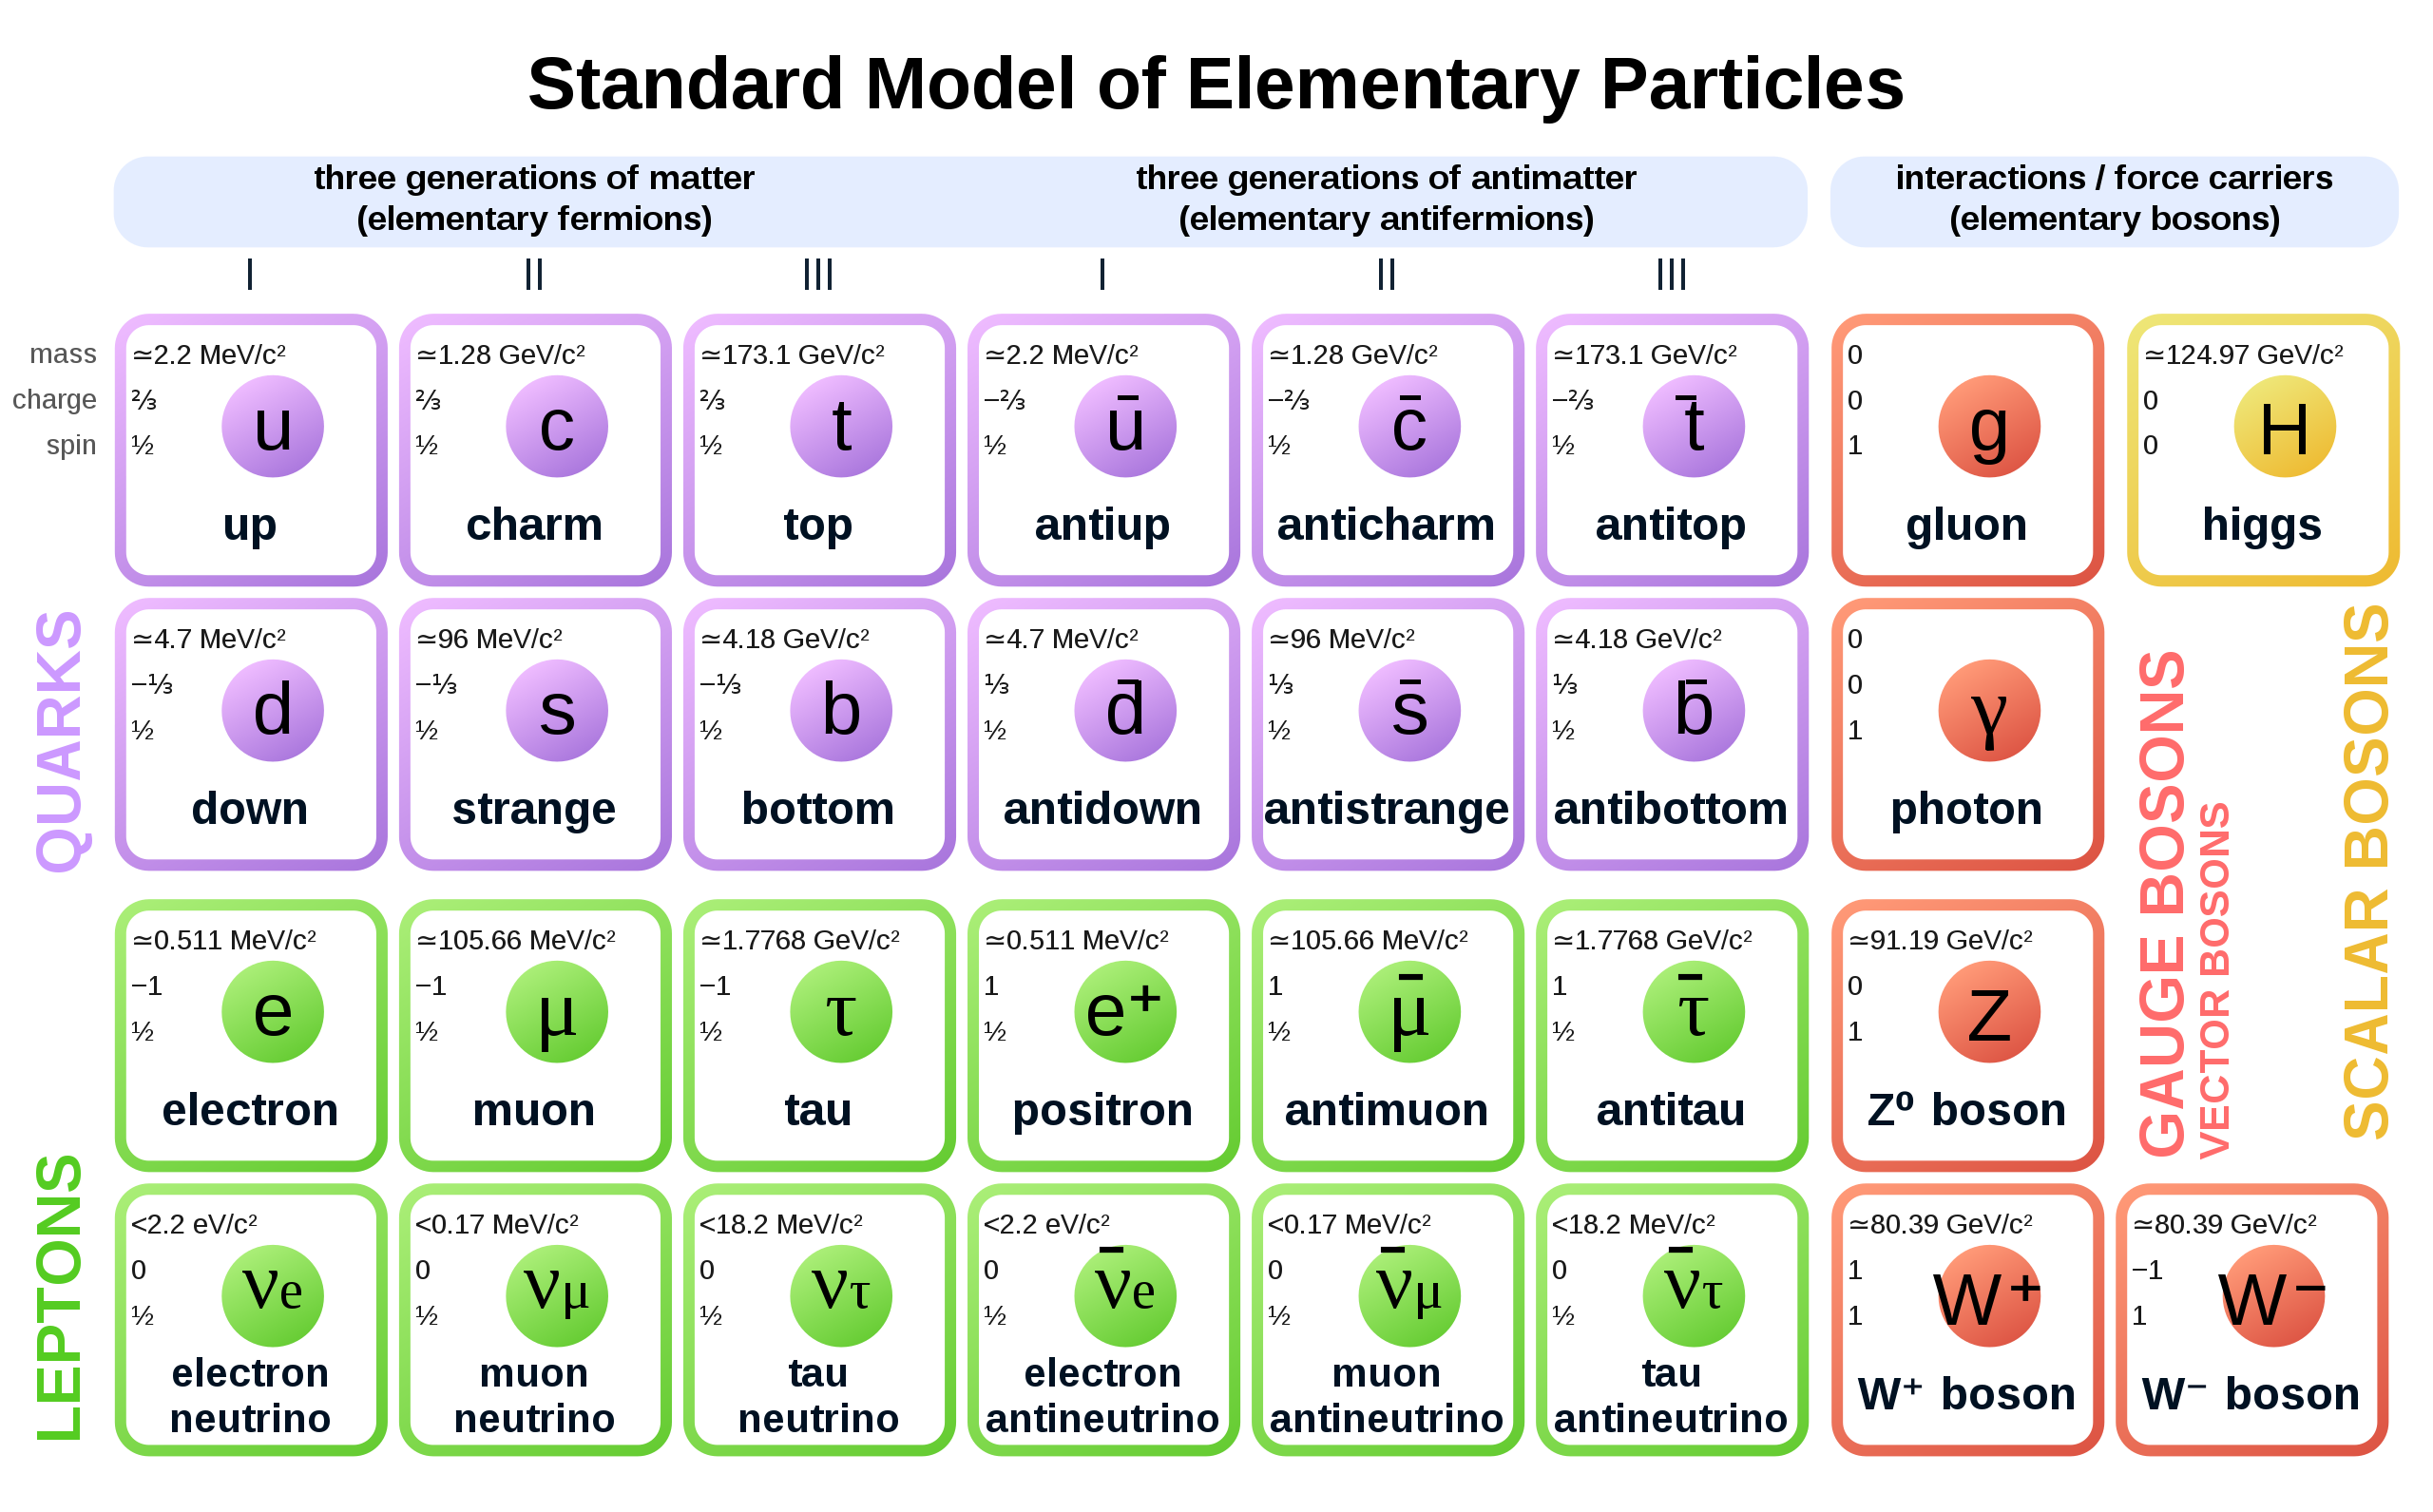
\includegraphics[width=0.99\textwidth]{figures/SMtable.png}
\caption[Summary of standard model fundamental particles]{Summary of SM fundamental particles. Figure source~\cite{SMtable}.
\label{fig:SMParticles}}
\end{figure}


\begin{figure}[t!]
\centering
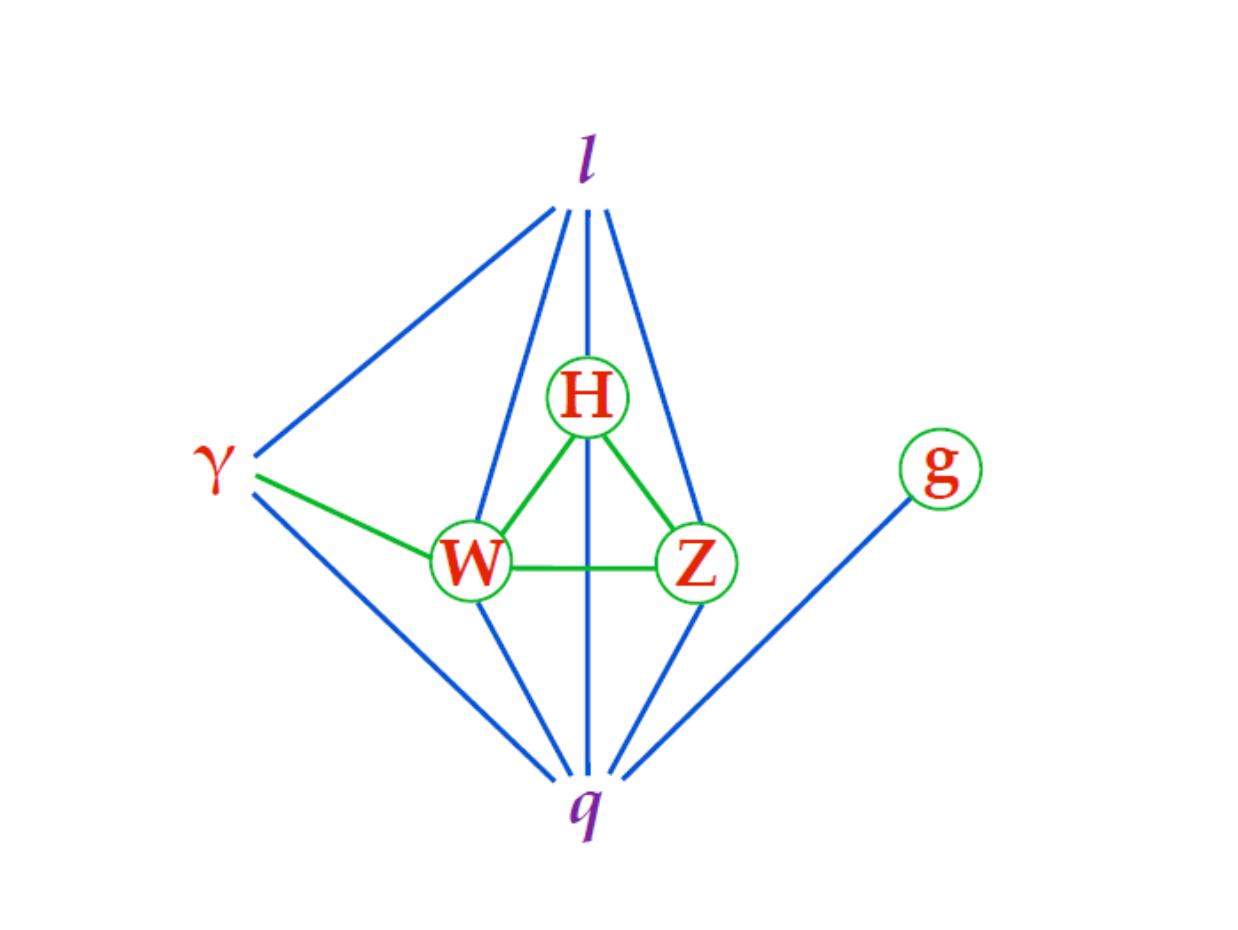
\includegraphics[width=0.99\textwidth]{figures/SM_coupling.png}
\caption[interactions between fundamental particles]
\label{fig:SMcoupling}}
\end{figure}

%
% LHC and experiments, Very brief physics summary
%
The Hadron Collider at CERN, Geneva, Switzerland is currently the largest and highest energy particle accelerator.
The LHC consists of a 27-km ring of superconducting magnets with a number of accelerating structures to boost the energy of the particles along the way.
The LHC can acclerate different types of beams and can produce proton-proton collisions, proton-lead collisions, and lead-lead collisions; however, the main operation mode provides proton-proton collisions.
%
The first proton-proton collisions were achieved by the LHC in 2010 at an energy of 3.5 teraelectronvolts (TeV) per beam, about four times the previous world record.
Over years, the collision energy was inceased and collision rate was also increased.
As of the year of 2024, the LHC collides protons at the center-of-mass energy of $\sqrt{s}=13.6$\TeV.
%
The beams in the LHC cross each other (called bunch crossing) at four points where the ALICE, ATLAS, CMS, and LHCb detectors are located.
%
Since the start of its operation, the experiments at the LHC provide a wide range of physics results and advanced our understanding of elementary particles and their interations.
%
Among various results from LHC experiments, the most signicant one is probably the discovery of the Higgs boson by the ATLAS and CMS experiments~\cite{ATLAS:2012yve,CMS:2012qbp,CMS:2013btf}
in the mass region of around 125\GeV, announced in July, 2012.
%
Since its discovery, the Higgs boson properties have been studied in detailed in different production and decay modes by both ATLAS and CMS experiments.
In addition, all LHC experiments have been making a wide range of measurements to probe elementary particle properties and performing searches for ``new physics`` beyond the SM, and so far no result show significant discrepancies with respect to expectations from the SM.

%
%
%
For these physics studies are not possible without the high performant particle detector.
Among four major LHC experiments, I worked on the CMS experiment.
The CMS detector is described in detail in these references~\cite{CMS,CMS:2023gfb}, and some important aspects are highlighted below.

%
%
%
\section{CMS Detector}

The CMS detector is one of the general purpose detectors at the LHC.
%
Similarly to many other general purpose detectors for hadron collider experiments, the CMS detector consits of multiple subsytems:
the solenoid magnet that bents charged particles, charged particle tracking detector, electromagnetic and hadron calorimeters, and muon detectors.
% Directly taken from
% https://twiki.cern.ch/twiki/bin/viewauth/CMS/Internal/PubDetector
% Long article version.
The central feature of the CMS apparatus is a superconducting solenoid of 6\unit{m} internal diameter, providing a magnetic field of 3.8\unit{T}. Within the solenoid volume are a silicon pixel and strip tracker, a lead tungstate crystal electromagnetic calorimeter (ECAL), and a brass and scintillator hadron calorimeter (HCAL), each composed of a barrel and two endcap sections. Forward calorimeters extend the pseudorapidity coverage provided by the barrel and endcap detectors. Muons are reconstructed in gas-ionization detectors embedded in the steel flux-return yoke outside the solenoid.
The central feature of the CMS apparatus is a superconducting solenoid of 6\unit{m} internal diameter, providing a magnetic field of 3.8\unit{T}.
%
Each of these detector components is described below.

\subsection{Tracker}

The inner tracker measures the momentum of the charged particles by tracking their path going through the magnetic field of the solenoid magnetic.
The less curved the path of the particle the higher its momentum.

The inner tracker tracks the path of the charged particle by measuring its position. The particle produces a tiny signal when passing through the inner tracker layers.
The pixel detector is the closest part of inner tracker to the beam line. It is a crucial component in reconstructing the path of the short-lived particles. It has four cylindrical layers and disks at either end. Each layer is composed of silicon modules  where the sized of pixel is $100\times150$ micrometer$^2$.

The silicon strips cover the pixel detector. Four inner barrel layers (TIB) with two inner endcaps (TID) and six outer barrel layer (TOB) with two endcaps (TED) closing off the tracker. Same as the pixel detector each layer is made of silicon modules that is optimized differently according to its place.

For a charged hadrons at a normal incident with $\pt < 20$\GeV the tracker measures the \pt with 1\% resolution. And the relative resolution will decrease with the increase of \pt to reach the energy resolution of the calorimeter.

\subsection{Superconducting Magnet}

The Superconducting magnet has a strong bending power that can separate the charged from neutral particles energy deposits inside the calorimeters. Also, we can measure the momentum of the charged particles knowing their bend trajectories.This large solenoid magnet covers the inner track and the two calorimeters and provide a $3.8$ T uniform magnetic field on the axial.  

\subsection{Electromagnetic Calorimeter}

The Electromagnetic Calorimeter allows is to measures the energies and the direction of electrons, photons by detecting a cluster of energy which corresponding to electromagnetic showers. The ECAL is a homogeneous calorimeter made of lead tungstate crystals. The crystals in the barrel cover a cylindrical layer while in the endcap they cover an x, y grid. Also, before either endcap disk there is a pre shower detector which serves two goals: finding the photons decayed from a neutral pion to discriminate them from prompt photons. And to by requiring a signal in the pre shower we can indicate the presence of an electron or a photon in the ECAL. The Intrinsic energy resolution of the ECAL barrelis measured with ECAL supermodel exposed to an electron beam. The photon energy resolution is excellent in the range $1-50$ \GeV which is a usual range of photons in jets.  
 

\subsection{Hadronic Calorimeter}

The main function of the HCAL is to detect the energy of the charged and neutral hadrons. A hadronic shower might start in the ECAL which will be fully absorbed in the HCAL. The corresponding clusters in the ECAL and  HCAL will be used to estimate their energies and directions of the hadrons. The HCAL is a sampling calorimeter has layers made of a brass absorber and a plastic scintillator tiles. It covers the ECAL with a barrel and two endcap disks. To extend the coverage Hadron forward calorimeters are placed at $11$ m of the interaction point. The combined (ECAL+HCAL) calorimeter energy resolution was measuredusing a pion test beam. 
 




\subsection{Muon Detector}

What is the main purpose/function of the tracker?
What is the geometry/structure/dimension?
Possibley some purformance measures.

%Here is the introduction to the topic.
%When chapters are referenced, the graduate school requires that words are used rather than numbers, e.g. ``Chapter One'' should be used instead of ``Chapter 1.''
%Use the command \verb|\cref| to reference chapters, for example \verb|\cref{chapter:ch1}|.
%The outline is as follows.
%\cref{chapter:ch2} is about paragraphs and sections.
%\cref{chapter:ch3} discusses footnotes and citations.
%\cref{chapter:ch4} presents floats.
%\cref{chapter:ch5} talks about lists.
%\cref{chapter:ch6} is the conclusion.

%=====================================
\chapter{The Standrad Model}
\label{chapter:ch2}
\section{Particle Flow Reconstruction}

Particle Flow is an advance algorithm that combines all the information gathered using all the detectors in the CMS to reconstruct and identify final state particles. These initial  reconstructed particles are known as PF candidates are electrons, photons, charged and neutral hadrons, and muons.

The PF uses the basic elements: first element is the tracks information coming from the inner tracker, and muon chamber tracks. The other element is energy deposits information from ECAL and the HCAL. In this way the PF could give a better description for the collision event.

The particle flow is done in stages : first stage Clustering calorimeter energy deposits, then Linking all the tracks and clusters based on spatial a proximity (cells are neighboring each other in eta -phi view). Where Links can form between : Tracks \& ECAL clusters, Tracks \& HCAL clusters, ECAL \& HCAL clusters, Inner tracks and muon tracks, Muon tracks \& ECAL clusters, Muon tracks \& HCAL clusters.

(Explain PF blocks and how to get  form that PF candidates)


\section{Particle Flow Reconstruction}
\section{Calorimeter Cluster Calibration}
This is another section.
There is likewise triple space between the preceding text and this section's title.
The observant reader will notice that there is a double space between the section's title and this text.

\subsection{Calorimeter Cluster Calibration}
This is a subsection.
Just like the section, there is a triple space between the preceding text and the subsection's title.
And just like the section, there is a double space between the subsection's title and the subsection's text.

\subsection{More Subsections}
Same concept. Triple Space before title and double space after.
Just To show a demonstration, some garbage text will follow this in a new paragraph.

\lipsum[1]

\subsubsection{Subsubsections}
Subsubsections can be used. Maps to Level 5 on the graduate school requirements.
And just like section and subsection, there is a triple space before the title.
But then everything changes.
There is a period after the title followed by 2 spaces.
But fear not, this behavior is defined in the template.

\subsubsection{Capitalization is not the same}
The grad school asked to use sentence cases instead of header cases in the title of the subsubsection.
Alvin believes this will change eventually.

\section{Stacked Headings}

% \stack % DO NOT USE THIS COMMAND

\subsection{This is a Stacked Heading}
In other words there is no text in the section, and we immediately introduce a subsection.
To get spacing right when sections are adjacent to subsections (when headings are stacked),
we once needed to use the \texttt{$\backslash$stack} command in between.
But this is now handled correctly byt the teplate (.cls) file. So do not use the stack command.
It is marked obsolete in the template.

In other words: there has to always be a triple space between the text preceding the subsection title and the subsection title.
In this particular case the text preceding the subsection title is the section title.
But the same rule applies: triple space.
Assuming this changes, adjust accordingly in the template.

\subsection{Deeper Stacks}

% \stack % DO NOT USE THIS COMMAND

\subsubsection{This is a Stacked Deep Heading}
Same as before, there is no text between the subsection above and the subsubsection here.
But fear not. 'Tis taken care of by the template.
Unless the requirements change, in which case I'm adjusting the 1em vspace in the template should be fine.

\subsubsection{But This is Not}
But it's fine. It's just another Level 5. Or if you prefer -- a subsubsection. Whichever you choose to call it.

%=====================================    
%\chapter{The LHC and the CMS experiment}
%\chapter{Introduction}
%\label{chapter:ch3}
%%%outline%% ECAL Cluster Calibration using Boosted Decision Tree

intro..
 talk about ECAL.
 introduce clustering algorithm in ECAL.  
 HLT vs offline PF ECAL cluster
 
 expand more on:
  the PF cluster calibration.
  how it was done perviously, and now in this thesis. 
  
computational details.. 
 3.1 Boosted Decision Tree (BDT)
  based semi-parametric regression.

 3.2 BDT training details  
  samples being used. for training and validation.
  Calibration procedure. Input and target variables to BDT.

 3.3 fitting function 
 Crystal Ball (CB) double function
 
Results and Discussion (might be moved to its chapter before conclusion) 
 compare old vs new corrections
 check the response, resolution in each regions EE. EB. add comments if the results has improved or stayed the same. 

%plots : showing (EB , EE regions) 
%-  mu vs pt (covering 3 ranges of pt gen particle) (EB , EE regions)
%-  mu vs eta (for each range of pt) (EB region)


\begin{figure}[ht]
%\centering
%\includegraphics[width=1in]{baylor}
\caption{EB - Full Readout : mu vs eta}
%\label{figure_example1}
\end{figure} 

\begin{figure}[ht]
%\centering
%\includegraphics[width=1in]{baylor}
\caption{EE - Full Readout : mu vs eta}
%\label{figure_example1}
\end{figure}

\begin{figure}[ht]
%\centering
%\includegraphics[width=1in]{baylor}
\caption{EB - Full Readout : mu vs pt}
%\label{figure_example1}
\end{figure}

\begin{figure}[ht]
%\centering
%\includegraphics[width=1in]{baylor}
\caption{EE - Full Readout : mu vs pt}
%\label{figure_example1}
\end{figure}

Include some set of stamp plots. (where we get mu & std from after fitting)

Now, for ZS set vs pt.

%\includegraphics[width=1in]{baylor}
\caption{EE - ZS Readout : mu vs pt}
%\label{figure_example1}
\end{figure}

\begin{figure}[ht]
%\centering
%\includegraphics[width=1in]{baylor}
\caption{EB - ZS Readout : mu vs pt}
%\label{figure_example1}
\end{figure}

HLT vs offline PF ECAL cluster

%1-plots :
%- (PF cluster offline E / PFC online E) vs pt
%- (PF cluster offline E / PFC online E) vs eta
%%%%%%%%%%%%%%%%%%%%%%%%%%%%%%%%%%%%%%%%%%%%%%%
\begin{figure}[ht]
%\centering
%\includegraphics[width=1in]{baylor}  
\caption{(PF cluster offline E / PFC online E) vs pt}
%\label{figure_example1}
\end{figure}

\begin{figure}[ht]
%\centering
%\includegraphics[width=1in]{baylor}
\caption{(PF cluster offline E / PFC online E) vs eta}
%\label{figure_example1}
\end{figure}
%%%%%%%%%%%%%%%%%%%%%%%%%%%%%%%%%%%%%%%%%%%%%%%%
%plots : 
%- (PF cluster offline corrected E / PFC online corrected  E) vs pt
%- (PF cluster offline corrected E / PFC online corrected  E) vs eta 
%%%%%%%%%%%%%%%%%%%%%%%%%%%%%%%%%%%%%%%%%%%%%%%
\begin{figure}[ht]
%\centering                                                                                                                                                                                                                                                                     
%\includegraphics[width=1in]{baylor}                                                                                                                                                                                                                                            
\caption{(PF cluster offline corrected E / PFC online corrected E) vs pt}
%\label{figure_example1}                                                                                                                                                                                                                                                        
\end{figure}~

\begin{figure}[ht]
%\centering 
%\includegraphics[width=1in]{baylor}
\caption{(PF cluster offline corrected E / PFC online corrected E) vs eta}
%\label{figure_example1}
\end{figure}~
%%%%%%%%%%%%%%%%%%%%%%%%%%%%%%%%%%%%%%%%%%%%%%%%

\section{Footnotes}

Ut vitae elit blandit, dictum augue aliquam, dictum neque. Integer sit amet eros
iaculis, interdum est quis, convallis metus. Maecenas vestibulum id lectus at
pellentesque.\footnote{This is a short footnote.} Aliquam dignissim, turpis eget
hendrerit ullamcorper, magna magna consectetur odio, pulvinar vestibulum felis
enim in ipsum. Donec cursus pharetra fringilla. Integer placerat ultrices libero
non porta. In id orci in ipsum aliquet rhoncus. Fusce ornare ornare
volutpat.\footnote{And this is a rather longer footnote that requires more than
one line, demonstrating the required single spacing.}

Vivamus vel tortor vel nibh aliquet egestas. Nullam rutrum porttitor placerat.
Pellentesque mattis ullamcorper sollicitudin. Nam et arcu nisi. Aenean hendrerit
odio non nisi ultricies, in consectetur odio rhoncus. Donec cursus consequat
tincidunt. Morbi pellentesque ut sem sit amet sollicitudin. Quisque bibendum
tincidunt quam, eu condimentum dui ullamcorper at.

\section{Citations}

Here is a citation \cite{fake1}, and here is another \cite{fake2}. Citations are
nice. Depending on your choice of bibliography, there may be different formats
you can use. For example, Chicago provides a family of short citation commands.

% this section still included with ch2.tex
%=====================================
\chapter{Particle Flow Algorithm and Calorimeter Cluster Calibration} 
%\chapter{Particle Flow Reconstruction and Calorimeter Cluster Calibration}
\label{chapter:ch3}
%%outline%% ECAL Cluster Calibration using Boosted Decision Tree

intro..
 talk about ECAL.
 introduce clustering algorithm in ECAL.  
 HLT vs offline PF ECAL cluster
 
 expand more on:
  the PF cluster calibration.
  how it was done perviously, and now in this thesis. 
  
computational details.. 
 3.1 Boosted Decision Tree (BDT)
  based semi-parametric regression.

 3.2 BDT training details  
  samples being used. for training and validation.
  Calibration procedure. Input and target variables to BDT.

 3.3 fitting function 
 Crystal Ball (CB) double function
 
Results and Discussion (might be moved to its chapter before conclusion) 
 compare old vs new corrections
 check the response, resolution in each regions EE. EB. add comments if the results has improved or stayed the same. 

%plots : showing (EB , EE regions) 
%-  mu vs pt (covering 3 ranges of pt gen particle) (EB , EE regions)
%-  mu vs eta (for each range of pt) (EB region)


\begin{figure}[ht]
%\centering
%\includegraphics[width=1in]{baylor}
\caption{EB - Full Readout : mu vs eta}
%\label{figure_example1}
\end{figure} 

\begin{figure}[ht]
%\centering
%\includegraphics[width=1in]{baylor}
\caption{EE - Full Readout : mu vs eta}
%\label{figure_example1}
\end{figure}

\begin{figure}[ht]
%\centering
%\includegraphics[width=1in]{baylor}
\caption{EB - Full Readout : mu vs pt}
%\label{figure_example1}
\end{figure}

\begin{figure}[ht]
%\centering
%\includegraphics[width=1in]{baylor}
\caption{EE - Full Readout : mu vs pt}
%\label{figure_example1}
\end{figure}

Include some set of stamp plots. (where we get mu & std from after fitting)

Now, for ZS set vs pt.

%\includegraphics[width=1in]{baylor}
\caption{EE - ZS Readout : mu vs pt}
%\label{figure_example1}
\end{figure}

\begin{figure}[ht]
%\centering
%\includegraphics[width=1in]{baylor}
\caption{EB - ZS Readout : mu vs pt}
%\label{figure_example1}
\end{figure}

HLT vs offline PF ECAL cluster

%1-plots :
%- (PF cluster offline E / PFC online E) vs pt
%- (PF cluster offline E / PFC online E) vs eta
%%%%%%%%%%%%%%%%%%%%%%%%%%%%%%%%%%%%%%%%%%%%%%%
\begin{figure}[ht]
%\centering
%\includegraphics[width=1in]{baylor}  
\caption{(PF cluster offline E / PFC online E) vs pt}
%\label{figure_example1}
\end{figure}

\begin{figure}[ht]
%\centering
%\includegraphics[width=1in]{baylor}
\caption{(PF cluster offline E / PFC online E) vs eta}
%\label{figure_example1}
\end{figure}
%%%%%%%%%%%%%%%%%%%%%%%%%%%%%%%%%%%%%%%%%%%%%%%%
%plots : 
%- (PF cluster offline corrected E / PFC online corrected  E) vs pt
%- (PF cluster offline corrected E / PFC online corrected  E) vs eta 
%%%%%%%%%%%%%%%%%%%%%%%%%%%%%%%%%%%%%%%%%%%%%%%
\begin{figure}[ht]
%\centering                                                                                                                                                                                                                                                                     
%\includegraphics[width=1in]{baylor}                                                                                                                                                                                                                                            
\caption{(PF cluster offline corrected E / PFC online corrected E) vs pt}
%\label{figure_example1}                                                                                                                                                                                                                                                        
\end{figure}~

\begin{figure}[ht]
%\centering 
%\includegraphics[width=1in]{baylor}
\caption{(PF cluster offline corrected E / PFC online corrected E) vs eta}
%\label{figure_example1}
\end{figure}~
%%%%%%%%%%%%%%%%%%%%%%%%%%%%%%%%%%%%%%%%%%%%%%%%

\section{Footnotes}

Ut vitae elit blandit, dictum augue aliquam, dictum neque. Integer sit amet eros
iaculis, interdum est quis, convallis metus. Maecenas vestibulum id lectus at
pellentesque.\footnote{This is a short footnote.} Aliquam dignissim, turpis eget
hendrerit ullamcorper, magna magna consectetur odio, pulvinar vestibulum felis
enim in ipsum. Donec cursus pharetra fringilla. Integer placerat ultrices libero
non porta. In id orci in ipsum aliquet rhoncus. Fusce ornare ornare
volutpat.\footnote{And this is a rather longer footnote that requires more than
one line, demonstrating the required single spacing.}

Vivamus vel tortor vel nibh aliquet egestas. Nullam rutrum porttitor placerat.
Pellentesque mattis ullamcorper sollicitudin. Nam et arcu nisi. Aenean hendrerit
odio non nisi ultricies, in consectetur odio rhoncus. Donec cursus consequat
tincidunt. Morbi pellentesque ut sem sit amet sollicitudin. Quisque bibendum
tincidunt quam, eu condimentum dui ullamcorper at.

\section{Citations}

Here is a citation \cite{fake1}, and here is another \cite{fake2}. Citations are
nice. Depending on your choice of bibliography, there may be different formats
you can use. For example, Chicago provides a family of short citation commands.

%=====================================
\chapter{Electromagnetic Cluster Calibration Using Boosted Decision Tree}
\label{chapter:ch4}
%% Ch4:Hadronic Cluster Calibration UsinAg Graph Neural Network%% 

\section{Introduction to Graph Neural Network}
GNN is a type of NN that is used to process data that can be represented as graphs.
% https://en.wikipedia.org/wiki/Graph_neural_network
% check: A Gentle Introduction to Graph Neural Networks https://distill.pub/2021/gnn-intro/
% check: Basic Understanding of Neural Network Structure https://medium.com/@sarita_68521/basic-understanding-of-neural-network-structure-eecc8f149a23
% check: Epochs, Batch Size, Iterations https://www.sabrepc.com/blog/Deep-Learning-and-AI/Epochs-Batch-Size-Iterations
%=================================================

% Where GNN's are used in CMS?
%% For Calorimetry, In both ECAL & HCAL.

% what are NN?
% what are GNN?

% where GNN can be used in ECAL?
%% for superclustering "Particle reconstruction", particle identification (identify the flavor of the particle), energy regression. 

% when do we perform energy correction?
%% after superclusters are formed, energy corrections are applied.
%% this correction account for the energy lost in gaps and upstream material .. etc
%% currently this calibration is done using BDT with semiparametric regression. (this work is covered in previous chapter)
%% new ML algorithm developed DRN (to use low level inputs (rechits) instead of high level inputs (describe EM showers))

% Energy corrections using Dynamic Reduction Network?
%% input features (rechits) are transformed into high dimensional latent space.
%% Then graphs are dynamically generated in the latent space.
%% the graph convolution are performed (includes message passing)
%% the info is aggregated over the graph using clustering and pooling.
%% => input: Rechit features (E,x,y,z) => output: Predict probability density of energy correction value.
%% slide 16 has resolution plot that compare BDT to DRN calibration. (using photon gun simulation with ideal detector calibration)

% source: ML for calorimetry by Polina simkina

%================================================

% DRN architecture overview:
%..........................
%% 1. input: Rechits => inputNet (FCNN) *Fully Convolutional Network?*
%% 2. => Graph Generation (KNN) => EdgeConv => calculate edge weights => graph clustering (Graclus) => graph pooling (add)
%% 3. Global pool (max)
%% 4. outputNet => output (E pred)

% Training target?
%% minimize loss - [(E true- E pre)^/E true]

% DRN training parapmeters?
%% Input layers: 3
%% aggregation layers: 2
%=> *An aggregation layer is a crucial part of network architecture that connects the access layer to the core layer.
%=> It's also known as the distribution layer.
%=> The aggregation layer's main purpose is to increase network scalability and manage traffic*
%=> source: https://www.sciencedirect.com/topics/computer-science/aggregation-layer#:~:text=The%20aggregation%20layer%20is%20defined,with%20vPC%20in%20computer%20networks.
%% message passing layers:3
%=> *Message passing layers are permutation-equivariant layers mapping a graph into an updated representation of the same graph.
%=> Formally, they can be expressed as message passing neural networks (MPNNs)* source: https://en.wikipedia.org/wiki/Graph_neural_network#Message_passing_layers
%% output layers: 2, *why 2 instead of 1??*
%% hidden dimension: 64
%% batch size: 100
%=> Batch Size is among the important hyperparameters in Machine Learning.
%=> It is the hyperparameter that defines the number of samples to work through before updating the internal model parameters.
%=> source: https://medium.com/geekculture/how-does-batch-size-impact-your-model-learning-2dd34d9fb1fa
%% optimizer w/ constant learning reate of 0.001 AdamW
%=> check video https://www.youtube.com/watch?v=oWZbcq_figk to learn more about AdamW
%% model parameters: 62405
%% total events # training, # validation. 

% Rechits (input): slide 11
%.................
% where do we get the PF Rechits? 
%% for each event we get the desired PF candidate. then we get the corresponding elements in its PFBlock (tracks/cluster).
%% then we collect all the PFElemnets of pfc which formed form eithr ECAL or HCAL.
%% then from each element we get the corresponding cluster reference & associated "hitAndFractions" = RecHits => input in ML algo.
% what are the input features?
%% Rechit position (x vs y) (z, Energy)

% note: for diagnostic checks we compare total rechit energy
% Raw energy (total raw pf)  , Gen level energy (total true pf) - X axis
% ?? - Y axis (slide 13) ?? frequency ?
% ** still don't understand plots in slide 14 ( is it corrected vs True? , color? frequency?)

% Summary
%........
%% Hadron Calibration is challenging.
%% The used input for ML modle is Rechits which are a PF element.
%% Calibration for (charged PF hadrons) using DRN & Chi squar method is done.
%% more improvement in the response for EH tha  H. 

% source: PF hadron cluster calibration 26/2/2024
%================================================

% What are the technical details of the calibration data,
%........................................................
%% centrally generated (true, raw) and reconstructed single pion (- charged hadron) samples.
%% In CMSSW version 12_6_4 (We used) , GT (global target) 126X_mcRun3_2023_forPU65_v4 (after ECAL corrections)
%% E range (2-200) (200-500) GeV (FlatRandomEGunProducer ) + |eta|<3  & |Phi| < 3.14 range 
%%%*This Particle Gun will generate one or more particles,
%%%all coming from the same vertex (0,0,0) and uniformly distributed in the user-specified phi-, eta- and energy-range*
% source: https://twiki.cern.ch/twiki/bin/view/CMSPublic/SWGuideParticleGuns

% How calibration using chi squre method is done?
%................................................

% How is it done using DRN?
%.........................

% what is the motivation for offline calibration?
%...............................................
% when plotting the resolution vs true energy for EH hadrons we can see that
%% the resolution is non linear
%%%* A "non-linear resolution" in calorimetry calibration refers to a method where the calibration constants applied to a calorimeter's signal
%%% are not a simple linear function of energy, meaning the relationship between the measured signal and the actual deposited energy is not a straight line,
%%% but instead exhibits curvature, requiring a more complex mathematical model to accurately convert signals to energy values;
%%% this is often necessary to account for inherent non-linearities in the calorimeter response,
%%% like variations in shower development at different energy levels or non-uniformities within the detector itself. (AI answer google)

%%%*a "calorimeter response" refers to the measurable signal produced by a calorimeter when a particle is completely absorbed within it,
%%% essentially representing the energy of the incident particle as a detectable output,
%%% typically in the form of light or electrical charge generated by the secondary particles produced in the particle shower;
%%% it is essentially how much signal is generated per unit of energy deposited in the calorimeter, and can vary depending on the type of particle being absorbed.*

% => check more general info about calorimeters see talk Calorimeters Energy measurement

% using  Chi square method, what are the energy/ Pseudorapidity dependent calibrationss?
% .........................................................................
%%%* In statistics, minimum chi-square estimation is a method of estimation of unobserved quantities based on observed data.
% => source: https://en.wikipedia.org/wiki/Minimum_chi-square_estimation
%% Energy dependent calibration: slide 5 
%% EH hadrons: E(corrected):a* E(raw Ecal) + b*E(raw Hcal) + O(EH) 
%% H hadrons: E(corrected): c*E(raw Hcal) + O(H)
%%% * coeffiecent O: accounts for the energy lost beacuse of the energy thresholds of the clustering algorithm.
%%% * coeffiecent a,b,c could be estimated using a large sample of simulated particles
%%% after getting the coeffiecents we can apply the corrections on the raw ECAL & HCAL energies. 


% types of calibration?
%.....................
% => check pg 47 Source: calorimetry for particle physics

%%%* Absolute calibration of a calorimeter is a process that determines the constants needed to convert raw ADC codes into energy depositions
%%% in the calorimeter counters. The goal is to ensure accurate measurements of heat changes in chemical reactions or physical processes. (AI answer google)


%%%%%%%%%%%%%%%%%%%%%%%%%%%%%%%%%%%%%%%%%%%%%%%%%%% 
\section{HCAL Cluster Calibration using GNN}

Hadronic showers in the CMS detector have both electromagnetic and hadronic components.

These showers are not dully contained in the ECAL but extend to HCAL.

The detector response is different for EM and HAD componenets which lead to non linear energy response.

The reconstructed energy of hadrons is the sum if all reconstructed hits (offline, PF reconstruct the RAW data) from the ECAL and HCAL.

For a given bin of ture energy (PF also reconstruct generated data or MC data):

by fitting the distribution of total RAW energy with Gaussian we obtain mu and std deviation then use them to get:

Resolution (std/mu) : which is a measure of accuracy

and Response [(mu/E true) -1] : which is measurement of precision. (we can see that is not linear)

Energy Reconstruction using conventional method (chi square) vs DRN (based on GNN).

The work in this thesis is done for Run3 data. 


\subsection{Strategy}


\subsection{Samples used and Training Details}

Include DRN architecture overview here. We could include the Training target.  

DRN training parameters. this include: Inpute layers (3) .. etc.

Sample details: centrally produced GEN-SIM-RAW (two momentum range) and privately reconstructed in CMSSW.

Rechits used as input. (we could expand more on this detail)

\subsection{Validation}

80\% of the dataset used for taining and 20\% for validation.  

% source: Chirayu talk 26/2 % 
%%%%%%%%%%%%%%%%%%%%%%%%%%%%%%%%%%%%%%%%%%%%%%%%%%% 
\section{Results and Discussion}

we present the results of response and resolution (from DRN vs Chi2) in  both Barrel region and endcap region.  
  \subsection{EH Hadrons}
  \subsection{H hadrons} 

%%%%%%%%%%%%%%%%%%%%%%%%%%%%%%%%%%%%%%%%%%%%%%%%%%%
  % side notes: reviewing other materials

  % How is physics analysis is done at the LHC?
  %% to study particles like Higgs boson, we need to be able to reconstruct such an event from inside the detector.
  %% this means we need to reconstruct the possible final products of Higgs decay: photon & pair of muon (decay products of Z)
  %% other things we need to reconstruct to do other analysis: electrons, hadrons.

  % How can we reconstruct collision events from the detector signals?
  %% By using Particle flow algorithm we can get an event description.
  %% PF uses info from each cms sub detector to identify and reconstruct the final products that have interacted with the detector. (5 types of particles)
  %% PF uses different algorithms to first reconstruct the elements: tracks, clusters and then to link them to form the PF blocks.
  %% from these blocks we can get the list of the PF particle candidates that could be analyized further
  %to get Hight level objects that should look similar to the event initial products ex: jets, MET.

  % How hadrons deposit energy in the CMS?
  % Why the calibration of hadrons clusters is important?
  % What methods are used in calibrating the energy of hadrons clusters?
  % What architecture used in GNN?
  % How can we imporve the GNN method?
  % How can we validate the results of the GNN training?

  % summary:
  %% this work shows the promising imporvment in hadron cluster calibration by using GNN.
  %% Note: check the PF meetings to see the latest updates related to this work 2023-2024
  
  %=====================================================

  % hadronic showers?
  %% First hadron calorimetry was used in studying the cosmic ray spectrum 1950s.
  %% Hadronic showers are more complicated than EM showers. they are deeper and they extend to HCAL. 
  %% Large number of nuclear processes involved in generating these showers.
  %% HAD showers have electromagentic and hadronic components.
  %% some hadrons start showering in ECAL while others in HCAL.

  % How the energy of the hadron is estimated?
  %% to be continue: source chirayu talk

  
























%%%%%%%%%%%%%%%%%%%%%%%%%%%%%%%%%%%%%%%%%%%%%%%%%%%
%\section{Captions}
%Figures are funny. They are notably different from tables and therefore requires some explanation. Here are the rules:
%\begin{enumerate}
%\item The caption is below the image
%\item The caption is centered if it's short, ie one line. 
%\item But if the text spans multiple lines, then it's left-justified. 
%\end{enumerate}

%Figure~\ref{figure_example1} has a short caption, and
%Figure~\ref{figure_example2} has a longer caption, demonstrating the required
%single-spacing.

%\begin{figure}[ht]
%\centering
%\includegraphics[width=1in]{baylor}
%\caption{This is a caption for this figure}
%\label{figure_example1}
%\end{figure}

%Figures like tables are floats and can be positioned anywhere. 
%This author favors placing images at the top. 
%But to illustrate, figure~\ref{figure_example2} is placed at the bottom. 

%\begin{figure}[b]
%\centering
%\includegraphics[width=0.2\textwidth]{baylor}
%\caption[The short table of contents version]{An example of a longer figure
%caption that spans multiple lines and has a corresponding short version for the
%table of contents.}
%\label{figure_example2}
%\end{figure}

%\section{Tables}

%Table~\ref{table_fruit} and Table~\ref{table_silly} demonstrate tables. Table
%captions differ slightly from figure captions, in that they are \textit{always}
%supposed to be centered, even if they use multiple lines.

%\begin{table}[h]
%\centering
%\caption[Fruits by color]{\centering Fruits listed by their color. Note that
%captions differ from figure captions in that they are \textit{always} supposed
%to be centered, even if they use multiple lines.}
%\label{table_fruit}
%\begin{tabular}{rl}
%    \hline
%    Fruit & Color  \\  \hline
%    Orange & Orange \\
%    Blue & Blueberry \\
%    Red & Cherry \\
%    Green & Apple \\
%    Yellow & Banana \\
%    Purple & Eggplant \\
%    \hline
%\end{tabular}
%\end{table}

%Tables can be anywhere in the text. They should be referred to \textbf{before} they make an appearance. 
%Tables can be placed between text, top of page, or bottom of page. This author personally prefers bottom of page. 
%There has to be triple space before the table captions, double space between caption and table, and triple space after the table. 

%The intext table (table~\ref{table_silly}) might look like it has more space after the table and before the text
%But that's just because the last item on the table is a horizontal line. 

%At the bottom of this page, is an example of a table set to [b]. This demonstrates the prettiness available to us by using tables at the bottom. 
%Bottom tables rock. As do top tables. 
%\begin{table}[b]
%\centering
%\caption[A bottom table]{A botom table illustrated}
%\label{table_silly}
%\begin{tabular}{ccc}
%    \hline
%    A & B & C \\  \hline
%    1 & 2 & 3 \\
%    4 & 5 & 6 \\
%    7 & 8 & 9 \\
%    \hline
%\end{tabular}
%\end{table}

%Nam dui ligula, fringilla a, euismod sodales, sollicitudin vel, wisi. Morbi auc-
%tor lorem non justo. Nam lacus libero, pretium at, lobortis vitae, ultricies et, tellus.
%Donec aliquet, tortor sed accumsan bibendum, erat ligula aliquet magna, vitae ornare
%odio metus a mi. Morbi ac orci et nisl hendrerit mollis. Suspendisse ut massa. Cras
%nec ante. Pellentesque a nulla. Cum sociis natoque penatibus et magnis dis par-
%turient montes, nascetur ridiculus mus. Aliquam tincidunt urna. Nulla ullamcorper
%vestibulum turpis. Pellentesque cursus luctus mauris.

%\begin{table}[!t]
%  \centering
%  \caption{This is a Top Positioned Table}
%  \begin{tabular}{ l c c c c }
%    \hline
%    \multirow{2}{*}{Interface} &
%    \multicolumn{2}{c}{Completion Time} &
%    \multicolumn{2}{c}{Throughput} \\
    
%    {} & Mean & Stdev & Mean & Stdev \\ 
%    \hline
%    Mouse only & 74s & 5.19 & 4.33bps & 0.35 \\
%    Mouse \& speech & 114s & 9.74 & 4.58bps & 0.46 \\
%    Gestures only & 116s & 14.76 & 2.66bps & 0.40\\
%    Gestures \& Speech & 136s & 14.82 & 2.83bps & 0.49\\
%    \hline
%  \end{tabular}
%  \label{tab:ranking}
%\end{table}


%Nam dui ligula, fringilla a, euismod sodales, sollicitudin vel, wisi. Morbi auc-
%tor lorem non justo. Nam lacus libero, pretium at, lobortis vitae, ultricies et, tellus.
%Donec aliquet, tortor sed accumsan bibendum, erat ligula aliquet magna, vitae ornare
%odio metus a mi. Morbi ac orci et nisl hendrerit mollis. Suspendisse ut massa. Cras
%nec ante. Pellentesque a nulla. Cum sociis natoque penatibus et magnis dis par-
%turient montes, nascetur ridiculus mus. Aliquam tincidunt urna. Nulla ullamcorper
%vestibulum turpis. Pellentesque cursus luctus mauris.

%=====================================
\chapter{Hadronic Cluster Calibration Using Graph Neural Network}
\label{chapter:ch5}







%%%%%%%%%%%%%%%%%%%%%%%%%%%%%%%%%%%%%%%%%%%%%%%%%%%%%%%
%\section{Lists}

%Lists have several characteristics:

%\begin{itemize}
%\item Lists can contain items
%\item Lists can contain other lists
%\begin{itemize}
%\item Different depths have different bullets
%\item Different depths have different margins
%\end{itemize}
%\item Lists are easy
%\end{itemize}

%\section{Enumerations}

%A reasonable chapter layout for the thesis might be

%\begin{enumerate}
%\item Introduction
%\item Related Work
%\item Methodology
%\item Results and Analysis
%\item Conclusion
%\end{enumerate}


%=====================================
\chapter{Summary and Conclusion}
\label{chapter:ch7}
\input{chapters/ch7}

% Appendices (optional)
%\multipleappendices % Change to \oneappendix if you have only one appendix!

%\begin{appendices}

%\chapter{Tables}
%\label{appendix:appendixA}
%\input{appendices/appendixA}

%\chapter{Diagrams}
%\label{appendix:appendixB}
%\input{appendices/appendixB}

%\chapter{Plots}
%\label{appendix:appendixC}
%\input{appendices/appendixC}

%\end{appendices}

% Bibliography
% Use IEEEtranBaylorPhys; based on IEEEtran, modified by Kenichi Hatakeyama
\bibliographystyle{IEEEtranBaylorPhys}
\bibliography{thesis}

\end{document}
OB
B
